\documentclass[t,handout]{beamer}
\usepackage[utf8]{inputenc}
\usepackage[ngermanb]{babel}
\usepackage{listings}
\lstset{basicstyle=\tiny}
% \lstset{language=bash}
\definecolor{darkblue}{rgb}{0,0,.5}
\hypersetup{pdftex=true, colorlinks=true, breaklinks=true, linkcolor=darkblue, menucolor=darkblue, pagecolor=darkblue, urlcolor=darkblue}

\title{Taskwarrior -- What's next?}
\subtitle{Task management on the commandline}
% \author[Deimeke, Dirk]{Dirk Deimeke}
\author{Dirk Deimeke}
% \institute[Ubucon 2011]{Deutsche Ubuntu Konferenz 2011}
\institute{Ubucon 2011}
% \date[16.10.2011]{16. Oktober 2011}
\date{October 2011}
\titlegraphic{
\includegraphics[width=3cm,height=3cm]{tw-xxl}}
\subject{Taskwarrior}
\keywords{taskwarrior, task, management, commandline, getting things done}

\setbeamercovered{transparent}

\pgfdeclareimage[width=5mm]{tw-logo}{tw-xl}

%%%%%%%%%%%%%%%%%%%%%%%%%%%%%%%%%%%%%%%%%%%%%%%%%%%%%%%%%%%%%%%%%%%%%%%
%
% LaTeX-Template for Taskwarrior by Dominik Wagenführ
% http://www.deesaster.org/
%
% Creative Commons Attribution-ShareAlike 4.0 (CC-BY-SA 4.0)
% https://creativecommons.org/licenses/by-sa/4.0/
%
%%%%%%%%%%%%%%%%%%%%%%%%%%%%%%%%%%%%%%%%%%%%%%%%%%%%%%%%%%%%%%%%%%%%%%%

%%%%%%%%%%%%%%%%%%%%%%%%%%%
% Layout - Start
%%%%%%%%%%%%%%%%%%%%%%%%%%%


\setbeamertemplate{navigation symbols}{}

\useinnertheme{default}
\useoutertheme{infolines}
\usefonttheme{structurebold}

\newlength{\boxwidth}
\setlength{\boxwidth}{121px}
\setbeamertemplate{headline}{%
\begin{beamercolorbox}[dp=3px,ht=6px,wd=\boxwidth,center]{palette tertiary}%
\insertauthor\ (\insertinstitute)%
\end{beamercolorbox}%
\vskip-9px\hskip\boxwidth
\begin{beamercolorbox}[dp=3px,ht=6px,wd=\boxwidth,center]{palette secondary}%
\inserttitle%
\end{beamercolorbox}%
\begin{beamercolorbox}[dp=3px,ht=6px,wd=\boxwidth,right]{palette primary}%
\insertdate\hskip15px\insertframenumber\,/\,\inserttotalframenumber\hspace*{8px}
\end{beamercolorbox}%
}
\setbeamertemplate{footline}{}

%%%%%%%%%%%%%%%%%%%%%%%%%%%
% Colors - Start
%%%%%%%%%%%%%%%%%%%%%%%%%%%

\definecolor{basecolor}{gray}{0.2}
\definecolor{mittelgrau}{gray}{0.4}
\definecolor{hellgrau}{gray}{0.93}
\definecolor{gelb}{rgb}{1.0,1.0,0.75}

% infolines color
\setbeamercolor{palette primary}{fg=white,bg=mittelgrau}
\setbeamercolor{palette secondary}{fg=white,bg=basecolor}
\setbeamercolor{palette tertiary}{fg=white,bg=black}

% frame and title color
\setbeamercolor{frametitle}{fg=white,bg=basecolor}
\setbeamercolor{titlelike}{fg=white,bg=basecolor}
\setbeamerfont{frametitle}{series=\bfseries}

% TOC color
\setbeamercolor{section in toc}{fg=basecolor}

% text color
\setbeamercolor{normal text}{fg=black,bg=white}

% item color
\setbeamercolor{item}{fg=basecolor}
\setbeamercolor{itemize item}{fg=black}

% block color
\setbeamercolor{block title}{fg=black,bg=gelb}
\setbeamercolor{block body}{fg=black,bg=gelb}

% block alert color
\setbeamercolor{block title alerted}{fg=black,bg=gelb}
\setbeamercolor{block body alerted}{fg=black,bg=gelb}

% block example color
\setbeamercolor{block title example}{fg=black,bg=gelb}
\setbeamercolor{block body example}{fg=black,bg=gelb}

\setbeamertemplate{frametitle}{%
\vskip-1px%
\begin{beamercolorbox}[wd=363px,ht=20px,dp=12px]{frametitle}
\usebeamerfont{frametitle}%
\usebeamercolor{frametitle}%
\vspace*{-5px}\hspace*{10px}
\includegraphics[width=24px,height=24px]{tw-xl.png}\\
\vspace*{-20px}\hspace*{40px}\insertframetitle%
\end{beamercolorbox}
}

%%%%%%%%%%%%%%%%%%%%%%%%%%%
% Colors - Stop
%%%%%%%%%%%%%%%%%%%%%%%%%%%

%%%%%%%%%%%%%%%%%%%%%%%%%%%%%%%%%%%%%%%%%%%%%%%%%%%%%%%%%%%%%%%%%%%%%%%

\begin{document}

\frame{\titlepage}

% \logo{\pgfuseimage{tw-logo}}

\frame{\frametitle{Content}\tableofcontents}

\section{Introduction} 
\parskip1ex

\frame{\frametitle{Dirk Deimeke (that's me)}
\begin{itemize}
	\item Maried, two dogs
	\item Born in Wanne-Eickel
	\item Living in Grüt (2008 emigrated to Switzerland)
	\item Senior Unix Systems Administrator in Zürich
	\item More \url{http://d5e.org/}
\end{itemize}
}

\frame{\frametitle{Dirk Deimeke (Ubuntu)}
\begin{itemize}
	\item President of German Ubuntu association \href{http://verein.ubuntu-de.org}{ubuntu Deutschland e. V.}
	\item Official point of contact for the \href{http://loco.ubuntu.com/teams/ubuntu-de-locoteam}{German LoCo-Team}
	\item Member of \href{http://loco.ubuntu.com/teams/ubuntu-swiss-users}{Swiss LoCo-Team}
	\item Ubuntu Member
	\item More \url{http://d5e.org/ubuntu} (German) or \url{https://wiki.ubuntu.com/DirkDeimeke} (English)
\end{itemize}
}

\frame{\frametitle{Dirk Deimeke (Taskwarrior)}
\begin{itemize}
	\item I first saw Taskwarrior at Ubucon 2009 in a lightning talk of \href{http://f.ederi.co/}{Federico Hernandez}, one of the core developpers. \pause
	\item Started to use it in the beginning of 2010. \pause
	\item Still enthusiastic about it! ;-) \pause
	\item In the middle of 2010 I joined the \href{http://taskwarrior.org/wiki/Credits}{Taskwarrior Core Team}
	\item I like working in an international team (Watertown (Massachusetts, USA), Gothenburg (West Gothland, Sweden), Braunschweig, (Lower Saxony, Germany), Richmond (Virginia, USA), Bonn (North Rhine-Westphalia, Germany), Toronto (Ontario, Canada), Gruet (Zurich, Switzerland))
	\item \url{http://taskwarrior.org/}
	\item \url{http://d5e.org/taskwarrior} (German) own blog-articles about Taskwarrior
\end{itemize}
}

\frame{\frametitle{About this session}
\begin{itemize}
\item \textbf{What is this all about?} \\
This is about Taskwarrior, an efficient tool for task management. Techniques for time management are not part of this session. \pause 
\item \textbf{Why are the slides in English?} \\
Taskwarrior is an international project. \pause
\item \textbf{Why do you use the beta-Version?} \\
With Taskwarrior 2.0.0 a new syntax will be introduced. \pause
\end{itemize}

\begin{alertblock}{Attention!}
\begin{itemize}
    \item This workshop is not a lecture, I want to do this together with you.
    \item Ask your questions if you have some!
\end{itemize}
\end{alertblock}
}

\frame{\frametitle{Reasons for Taskwarrior}
Taskwarrior
\begin{itemize}
	\item is easy to learn.
	\item grows along with the work.
	\item is unbelievably powerful.
	\item is very fast.
	\item is easily extensible. 
	\item is platform independent:
	\begin{itemize}
		\item Most flavours of Unix and Linux, including Mac OS X and Ubuntu (PPA exists)
		\item Windows with Cygwin
		\item via SSH from my mobile
		\item \url{http://taskwarrior.org/w/Platforms}
	\end{itemize}
	\item is actively developed.
	\item can be influenced by users (feature requests).
	\item has excellent and very friendly support.
\end{itemize}
}

\section{Installation}

\begin{frame}[fragile]
\frametitle{Installation with package management}
\textbf{All download-addresses} \\
\url{http://taskwarrior.org/download} \pause

\textbf{Since Maverick Meerkat in Universe} \\
(Unfortunately version is behind recent)
\begin{lstlisting}
$ sudo apt-get install task
\end{lstlisting} \pause

\textbf{There is a PPA with the most recent version} \\
\url{https://launchpad.net/~ultrafredde/+archive/ppa}
\begin{lstlisting}
$ sudo add-apt-repository ppa:ultrafredde/ppa
$ sudo apt-get update
$ sudo apt-get install task
\end{lstlisting}
\end{frame}

\begin{frame}[fragile]
\frametitle{Installation from source}
The Meta-Package \texttt{build-essential} and \texttt{cmake} are all you need to compile.
\begin{lstlisting}
$ sudo apt-get install build-essential cmake
\end{lstlisting}
Download of recent version
\begin{lstlisting}
$ curl -O http://www.taskwarrior.org/download/task-2.0.0.beta3.tar.gz
$ # or wget http://www.taskwarrior.org/download/task-2.0.0.beta3.tar.gz
\end{lstlisting}
Untar and compile
\begin{lstlisting}
$ tar task-2.0.0.beta3.tar.gz
$ cd task-2.0.0.beta3
$ cmake .
$ make
$ sudo make install
\end{lstlisting}
The last command installs Taskwarrior to /usr/local.
\end{frame}

\begin{frame}[fragile]
\frametitle{Installation from source with target directory}
If you don't have root permissions or in case you want to use other directories, this is possible as well. \\
(No speciality of Taskwarrior).
\begin{lstlisting}
$ cmake -DCMAKE_INSTALL_PREFIX=/home/dirk/task-2.0.0.beta3 .
$ make
$ make install # without "sudo"
\end{lstlisting}
It makes sense to define the following three variables for the next steps. (The first one is not needed, I use it only for this topic to fit on one slide).
\begin{lstlisting}
$ taskdir=/home/dirk/task_2.0.0.beta3
$ export PATH=${taskdir}/bin:${PATH}
$ export LD_LIBRARY_PATH=${taskdir}/lib:${LD_LIBRARY_PATH}
$ export MANPATH=${taskdir}/man:${MANPATH}
\end{lstlisting}
\end{frame}

\begin{frame}[fragile]
\frametitle{Test of your installation}
\begin{lstlisting}
$ task version
A configuration file could not be found in /home/user

Would you like a sample /home/user/.taskrc created, so taskwarrior can proceed? (y/n) y

task 2.0.0.beta3 built for linux
Copyright (C) 2006 - 2011 P. Beckingham, F. Hernandez.

Taskwarrior may be copied only under the terms of the GNU General Public License, which may be found
in the taskwarrior source kit.

Documentation for taskwarrior can be found using 'man task', 'man taskrc', 'man task-tutorial', 'man
task-color', 'man task-sync', 'man task-faq' or at http://taskwarrior.org
\end{lstlisting}
\end{frame}

\begin{frame}[fragile]
\frametitle{Remove Taskwarrior}
\textbf{Package manager}
\begin{lstlisting}
$ apt-get purge task
\end{lstlisting}

\textbf{Sources}
\begin{lstlisting}
$ make uninstall
\end{lstlisting}
\end{frame}

\section{Simple ToDo-Lists}

\begin{frame}
\frametitle{A simple example, part 1}
\begin{center}
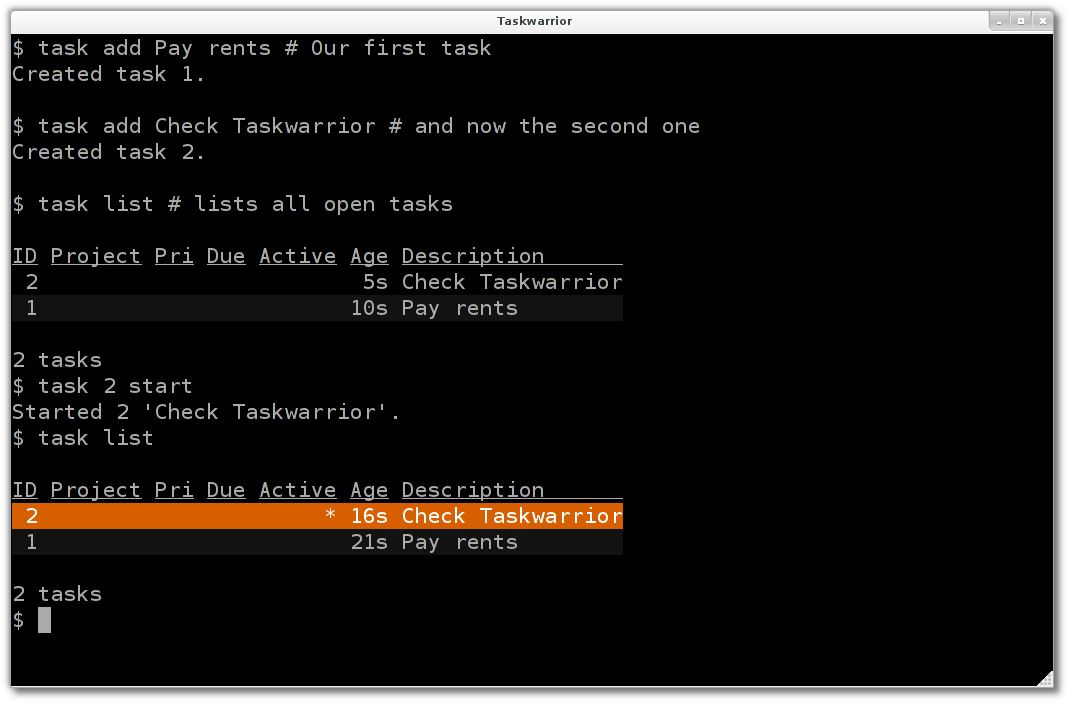
\includegraphics[width=10cm,height=7.5cm]{simple_example01.png}
\end{center}
\end{frame}

\begin{frame}
\frametitle{A simple example, part 2}
\begin{center}
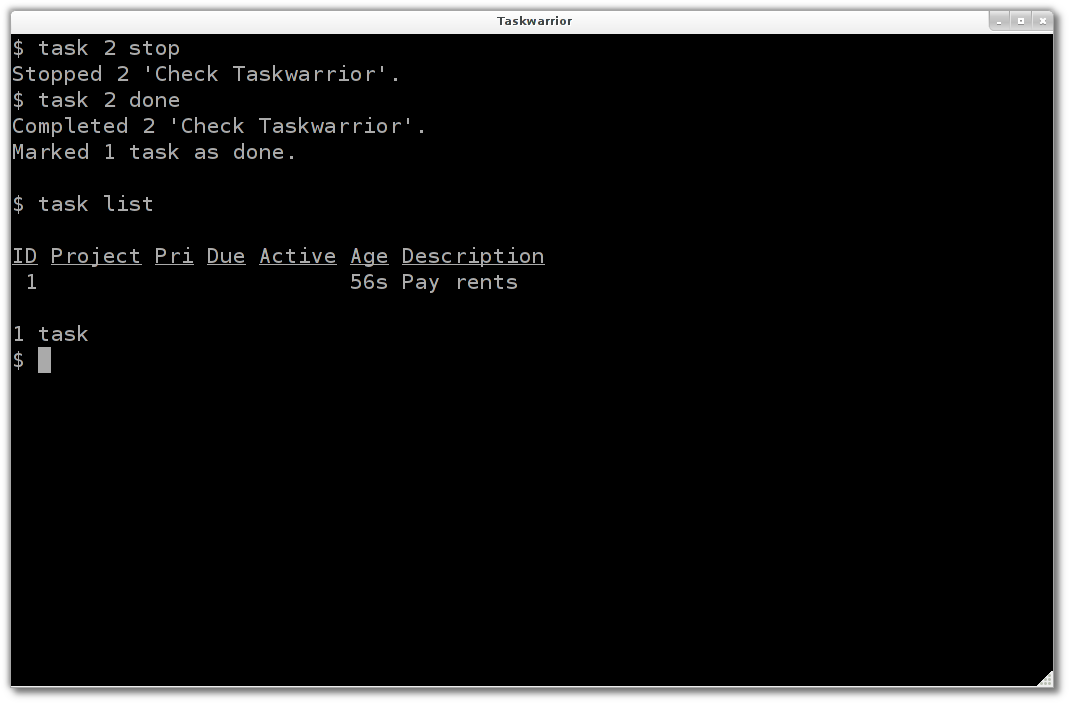
\includegraphics[width=10cm,height=7.5cm]{simple_example02.png}
\end{center}
\end{frame}

\begin{frame}
\frametitle{Commands so far}
\begin{itemize}
\item \textbf{task add} \\
Adds a new task to the task list. \pause
\item \textbf{task list} \\
Provides a standard listing of tasks. \pause
\item \textbf{task start} \\
Marks the specified tasks as started. \pause
\item \textbf{task stop} \\
Removes the start time from the specified task. \pause
\item \textbf{task done} \\
Marks the specified task as done.
\end{itemize}
\end{frame}

\frame{\frametitle{That's it!}
\begin{center}
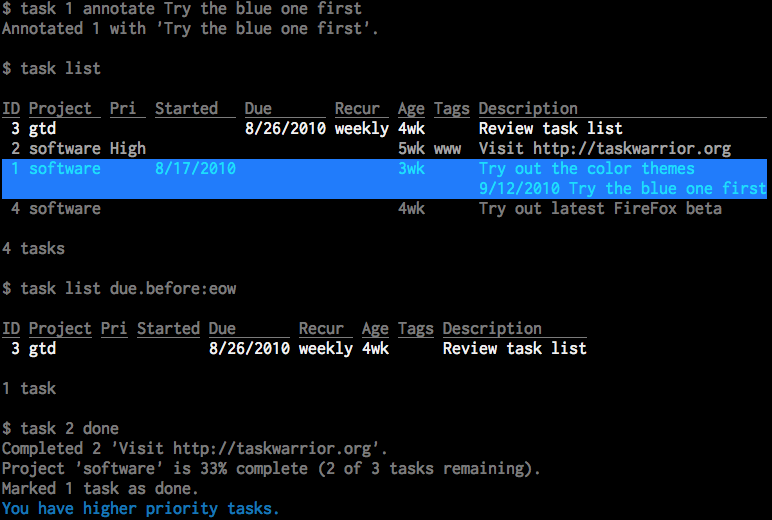
\includegraphics[width=6cm,height=4.5cm]{default-large.png}

\huge{Thanks for your attention!}

\normalsize{\href{mailto:dirk@deimeke.net}{dirk@deimeke.net}}

\url{http://taskwarrior.org/}
\end{center}
}

\section{General}

\frame{\frametitle{Just kidding ...}
\textbf{There is a lot more to explore.}

Even the commands from the last section are more mighty than they seem. \pause

\begin{itemize}
\item \textbf{task add {\tt<}mods{\tt>}}
\item \textbf{task {\tt<}filter{\tt>} list}
\item \textbf{task {\tt<}filter{\tt>} start {\tt<}mods{\tt>}}
\item \textbf{task {\tt<}filter{\tt>} stop {\tt<}mods{\tt>}}
\item \textbf{task {\tt<}filter{\tt>} done {\tt<}mods{\tt>}}
\end{itemize} \pause

To get an overview, take a look at the \href{http://www.taskwarrior.org/download/task-2.0.0.ref.pdf}{cheat sheet} (pdf, 145kB).
}

\begin{frame}
\frametitle{task {\tt<}filter{\tt>} command {\tt<}mods{\tt>}}
\begin{itemize} 
\item Is the basic usage of all task related write commands.
\item Write commands can operate on one task or a group of tasks or even on all tasks.
\item Every command maybe abbreviated up to the minimum that is necessary to identify a single command.
\item Filters can be anything from nothing to simple IDs further to regular expressions or Boolean constructs.
\item Modifications can be either a change of description, a change of dates or anything else that changes a task.
\item In our simple example we already used the write commands \textbf{add}, \textbf{done}, \textbf{start} and \textbf{stop}.
\end{itemize}
\end{frame}

\begin{frame}
\frametitle{Scripts}
\begin{center}
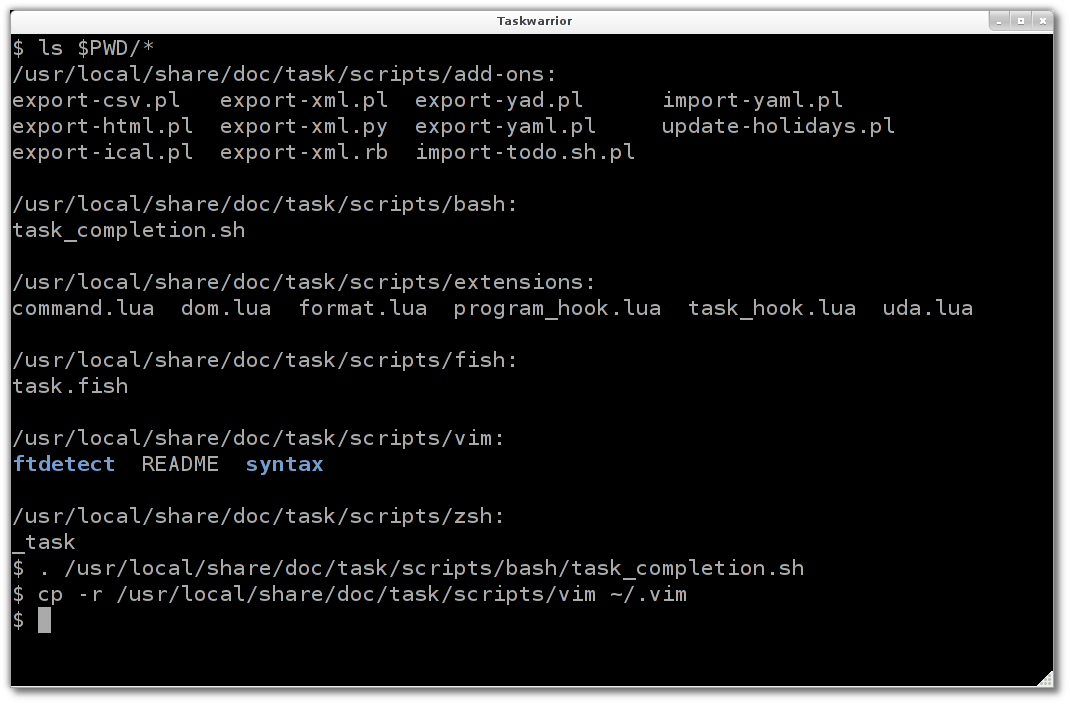
\includegraphics[width=10cm,height=7.5cm]{scripts.png}
\end{center}
\end{frame}

\begin{frame}
\frametitle{Most important commands}

These are the most important commands, just because I use them most ;-)

\begin{itemize}
\item \textbf{task {\tt<}filter{\tt>} modify} \\
The name says it, it modifies tasks according to the filter used. \pause
\item \textbf{task {\tt<}filter{\tt>} edit} \\
This starts your favourite editor with the tasks you want to change. \\
(Remember the syntax highlighting for vim?) \pause
\item \textbf{task undo} \\
Reverts the most recent change to a task. \pause
\item \textbf{task help} \\
Gives an overview of implemented commands and custom reports. \pause
\item \textbf{man task (taskrc, task-tutorial, task-color, task-faq, task-synch)} \\
Show the (almighty) man-page(s). Unlike the man-pages of many other 
programs they are extremely helpful and full of information and examples. 
Try them!
\end{itemize}
\end{frame}

\section{Working with dates}

\begin{frame}[fragile]
\frametitle{Dateformats -- from 'man taskrc'}
\begin{lstlisting}
m  minimal-digit month,   for example 1 or 12
d  minimal-digit day,     for example 1 or 30
y  two-digit year,        for example 09
D  two-digit day,         for example 01 or 30
M  two-digit month,       for example 01 or 12
Y  four-digit year,       for example 2009
a  short name of weekday, for example Mon or Wed
A  long name of weekday,  for example Monday or Wednesday
b  short name of month,   for example Jan or Aug
B  long name of month,    for example January or August
V  weeknumber,            for example 03 or 37
H  two-digit hour,        for example 03 or 11
N  two-digit minutes,     for example 05 or 42
S  two-digit seconds,     for example 07 or 47

The  string may also contain other characters to act as spacers,
or formatting.  Examples for other values of dateformat:

d/m/Y  would use for input and output 24/7/2009
yMD    would use for input and output 090724
M-D-Y  would use for input and output 07-24-2009

Examples for other values of dateformat.report:

a D b Y (V)  would do an output as "Fri 24 Jul 2009 (30)"
A, B D, Y    would do an  output  as  "Friday,  July  24, 2009"
vV a Y-M-D   would do an output as "v30 Fri 2009-07-24"
yMD.HN       would do an output as "110124.2342"
m/d/Y H:N    would do an output as "1/24/2011 10:42"
a  D  b  Y  H:N:S would do and output as "Mon 24 Jan 2011 11:19:42"
\end{lstlisting}
\end{frame}

\begin{frame}
\frametitle{Set dateformat}
\begin{center}
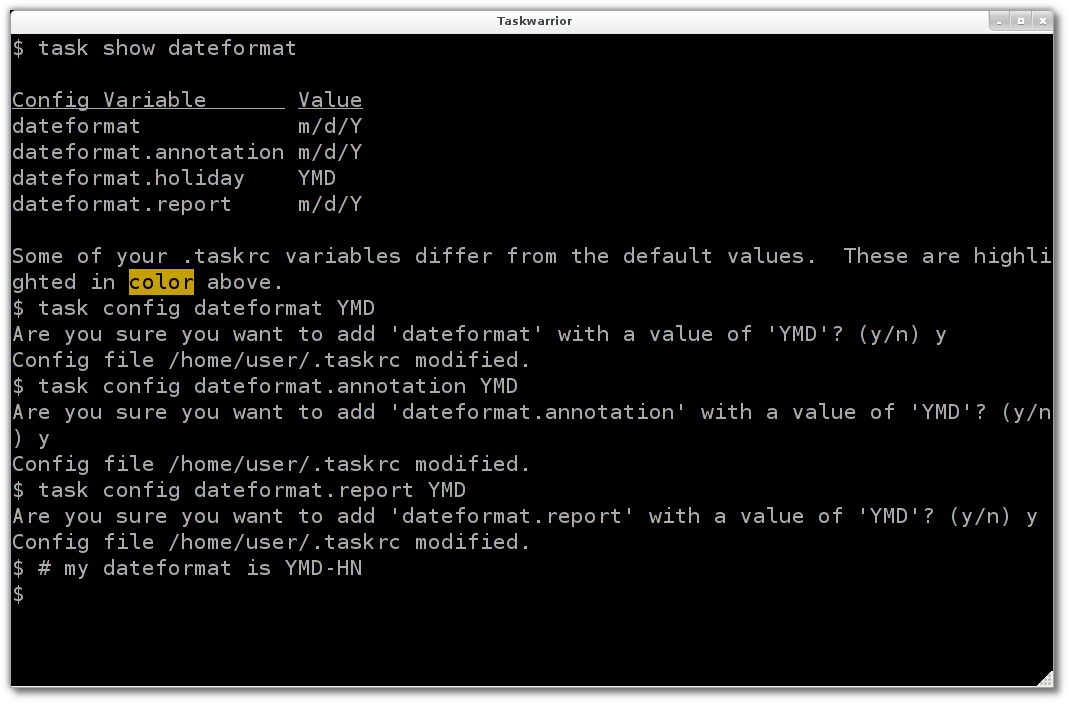
\includegraphics[width=10cm,height=7.5cm]{set_dateformat.png}
\end{center}
\end{frame}

\begin{frame}
\frametitle{Set weekstart}
\begin{center}
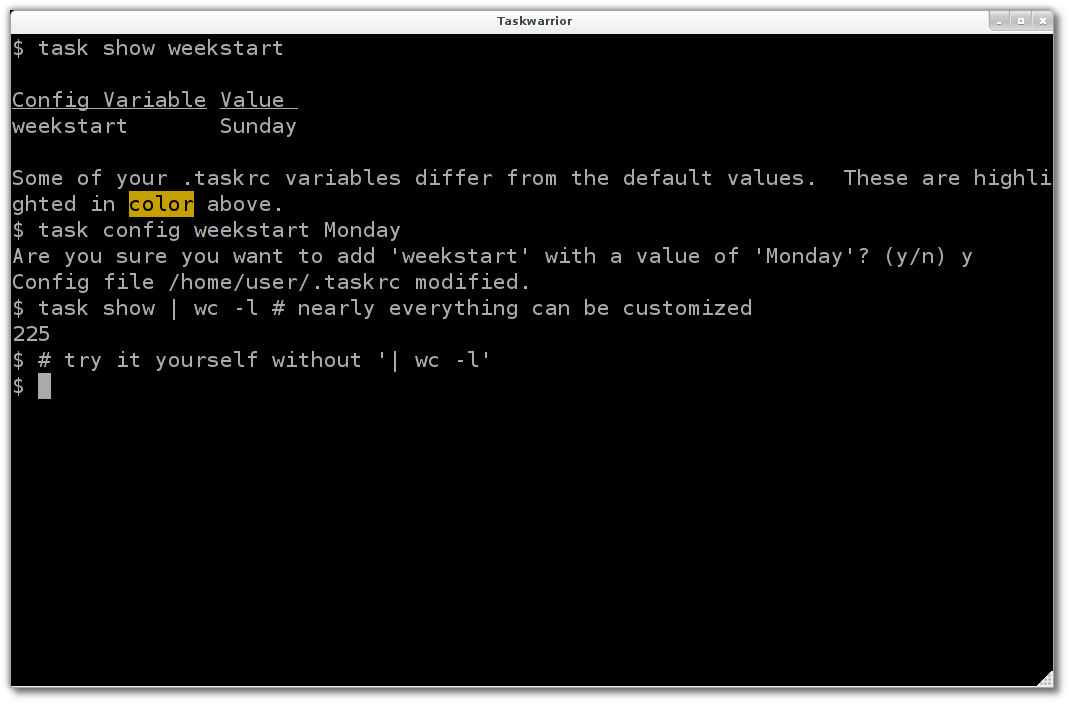
\includegraphics[width=10cm,height=7.5cm]{set_weekstart.png}
\end{center}
\end{frame}

\begin{frame}
\frametitle{Special dates (1)}
\begin{itemize}
\item \textbf{Relative wording} \\
task ... due:today \\
task ... due:yesterday \\
task ... due:tomorrow \\
\item \textbf{Day number with ordinal} \\
task ... due:23rd \\
task ... due:3wks \\
task ... due:1day \\
task ... due:9hrs \\
\item \textbf{At some point or later} \\
task ... wait:later
task ... wait:someday
This sets the wait date to 1/18/2038.
\end{itemize}
\end{frame}

\begin{frame}
\frametitle{Special dates (2)}
\begin{itemize}
\item \textbf{Start / end of (work) week, calendar week (according to settings of weekstart), month, quarter and year} \\
task ... due:sow \\
task ... due:eow \\
task ... due:soww \\
task ... due:eoww \\
task ... due:socw \\
task ... due:eocw \\
task ... due:som \\
task ... due:eom \\
task ... due:soq \\
task ... due:eoq \\
task ... due:soy \\
task ... due:eoy \\
\item \textbf{Next occurring weekday} \\
task ... due:fri
\end{itemize}
\end{frame}

\begin{frame}
\frametitle{Due and wait}
\begin{center}
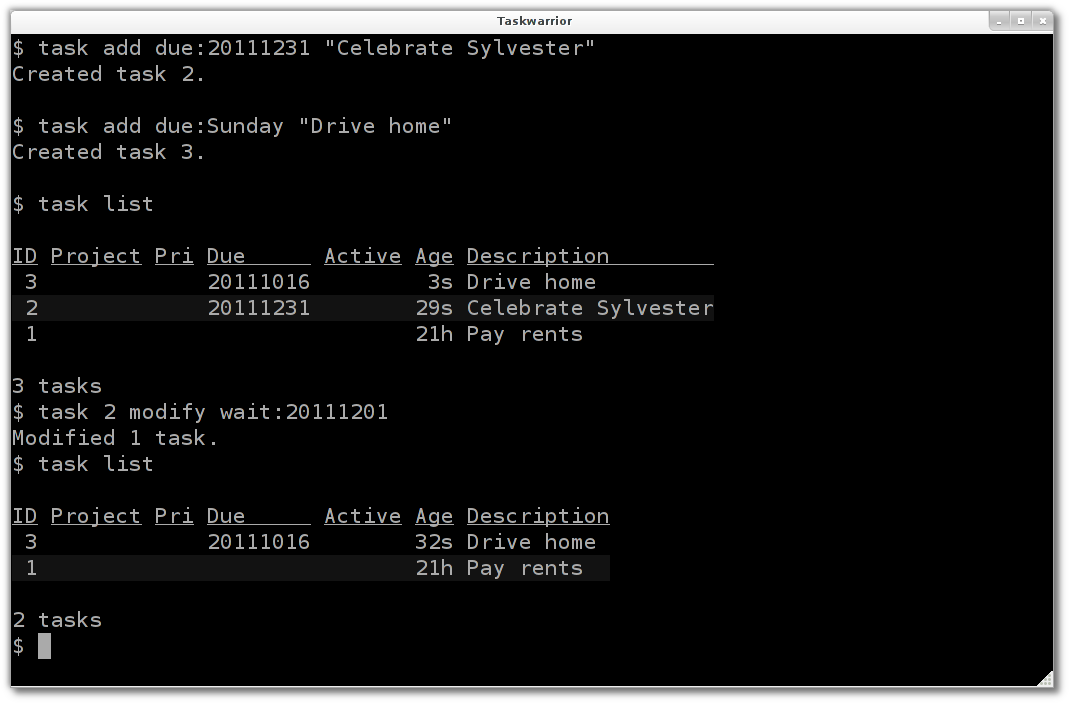
\includegraphics[width=10cm,height=7.5cm]{due_and_wait.png}
\end{center}
\end{frame}

\begin{frame}
\frametitle{Recurrence}
\begin{center}
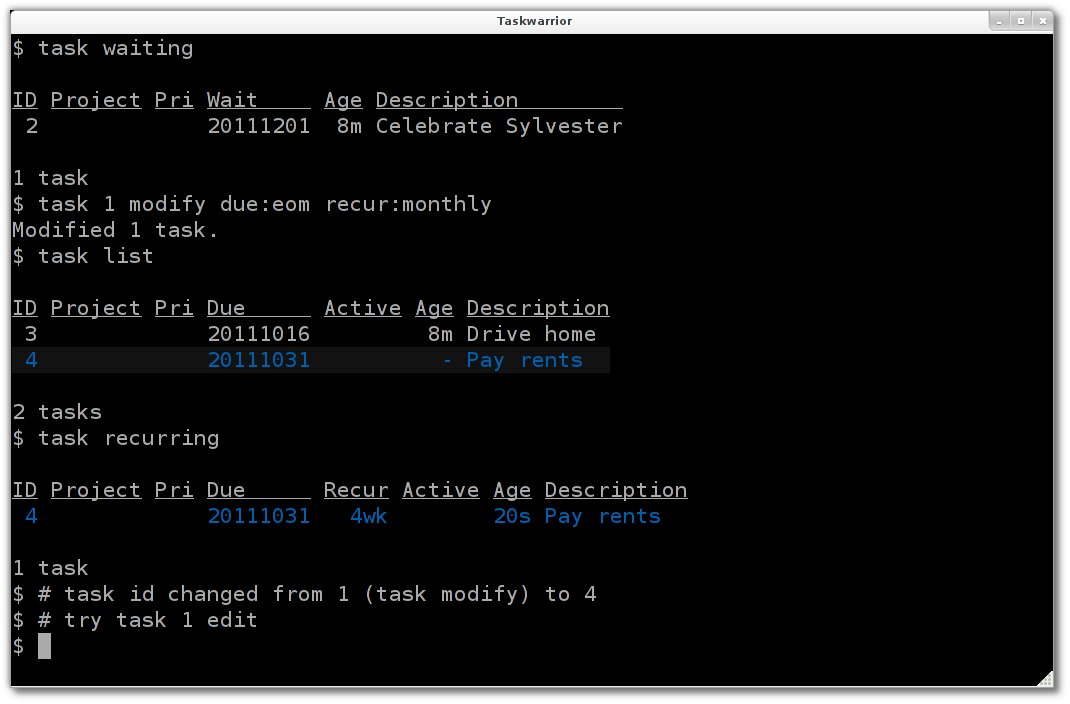
\includegraphics[width=10cm,height=7.5cm]{recur.png}
\end{center}
\end{frame}

\begin{frame}
\frametitle{Recurrence modifiers (1)}
\begin{itemize}
\item \textbf{hourly} \\
Every hour.
\item \textbf{daily, day, 1da, 2da, ...} \\
Every day or a number of days.
\item \textbf{weekdays} \\
Mondays, Tuesdays, Wednesdays, Thursdays, Fridays and skipping  weekend days.
\item \textbf{weekly, 1wk, 2wks, ...} \\
Every week or a number of weeks.
\item \textbf{biweekly, fortnight} \\
Every two weeks.
\item \textbf{monthly} \\
Every month.
\item \textbf{quarterly, 1qtr, 2qtrs, ...} \\
Every three months, a quarter, or a number of quarters.
\end{itemize}
\end{frame}

\begin{frame}
\frametitle{Recurrence modifiers (2)}
\begin{itemize}
\item \textbf{semiannual} \\
Every six months.
\item \textbf{annual, yearly, 1yr, 2yrs, ...} \\
Every year or a number of years.
\item \textbf{biannual, biyearly, 2yr} \\
Every two years.
\end{itemize}
\end{frame}

\begin{frame}
\frametitle{Until and entry}
\begin{center}
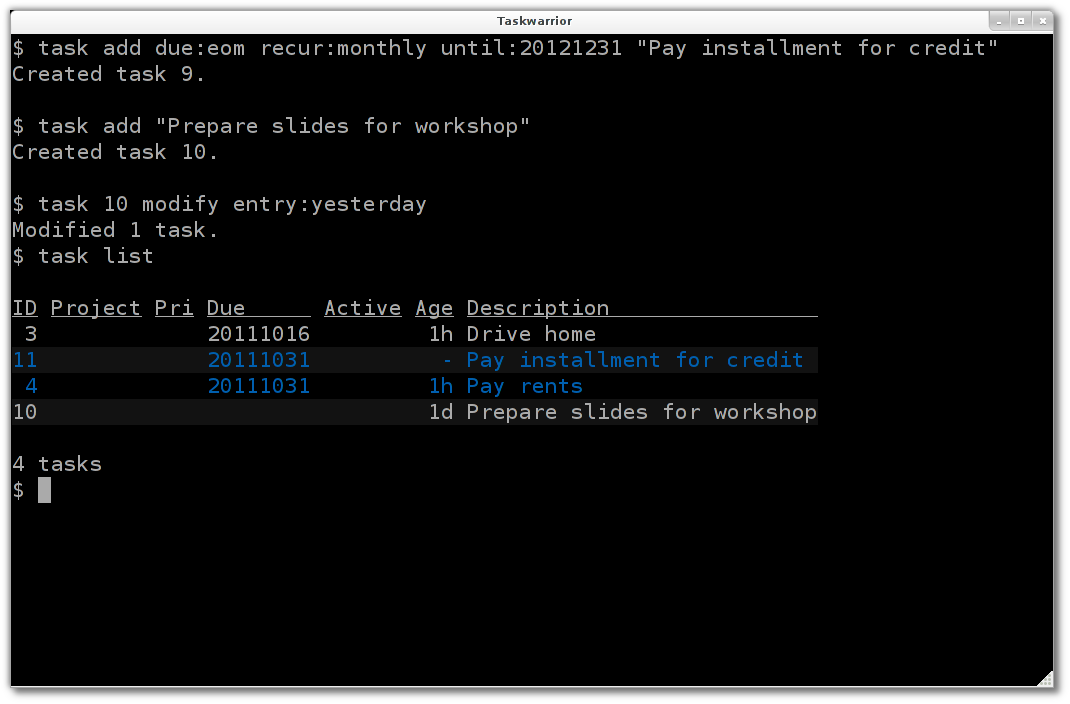
\includegraphics[width=10cm,height=7.5cm]{until_and_entry.png}
\end{center}
\end{frame}

\begin{frame}
\frametitle{Starting and stopping}
\begin{center}
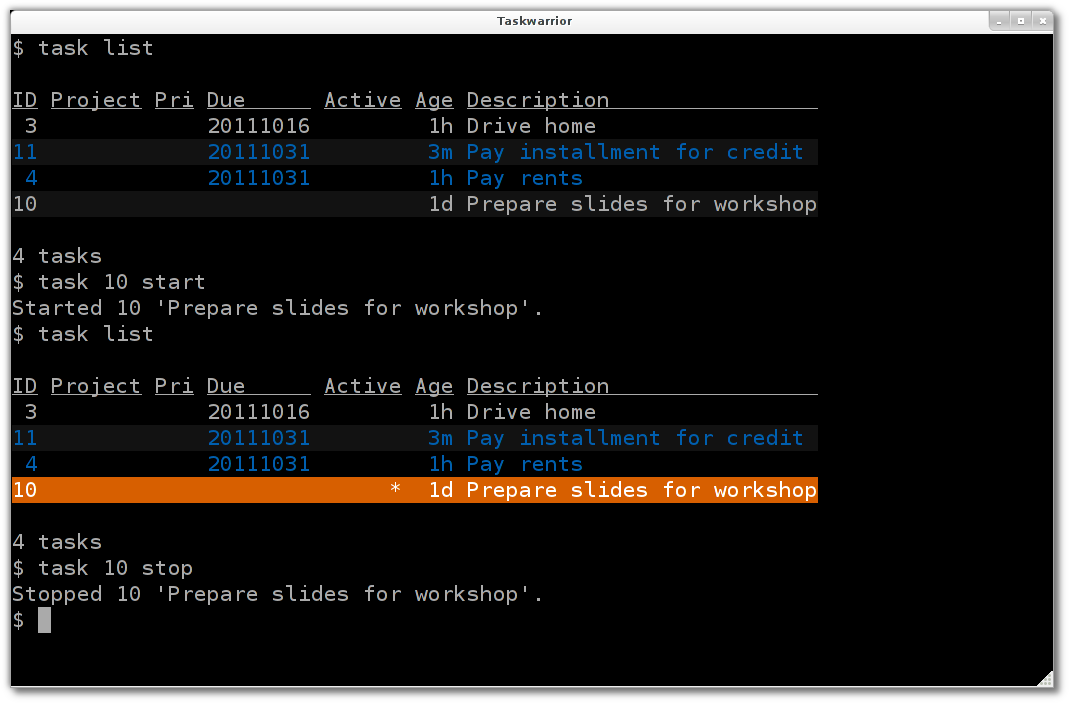
\includegraphics[width=10cm,height=7.5cm]{starting_and_stopping.png}
\end{center}
\end{frame}

\begin{frame}
\frametitle{Holiday}
\begin{alertblock}{Attention!}
Holiday has nothing in common with the German words "'Ferien"' or "'Urlaub"' (this would be vacation). (Public) Holiday means "'Feiertag"'.
\end{alertblock}

You can add holidays by either adding them via "'task config"' on the commandline or by adding them directly to the ~/.taskrc-File or by including an external holiday definition.

On \href{http://holidata.net/}{holidata.net} you find a growing list of holiday dates, licensed CC-BY and offered by volunteers. Service was introduced by the Taskwarrior team, who is responsible for hosting and conversion to different formats.
\end{frame}

\begin{frame}
\frametitle{Add holiday}
\begin{center}
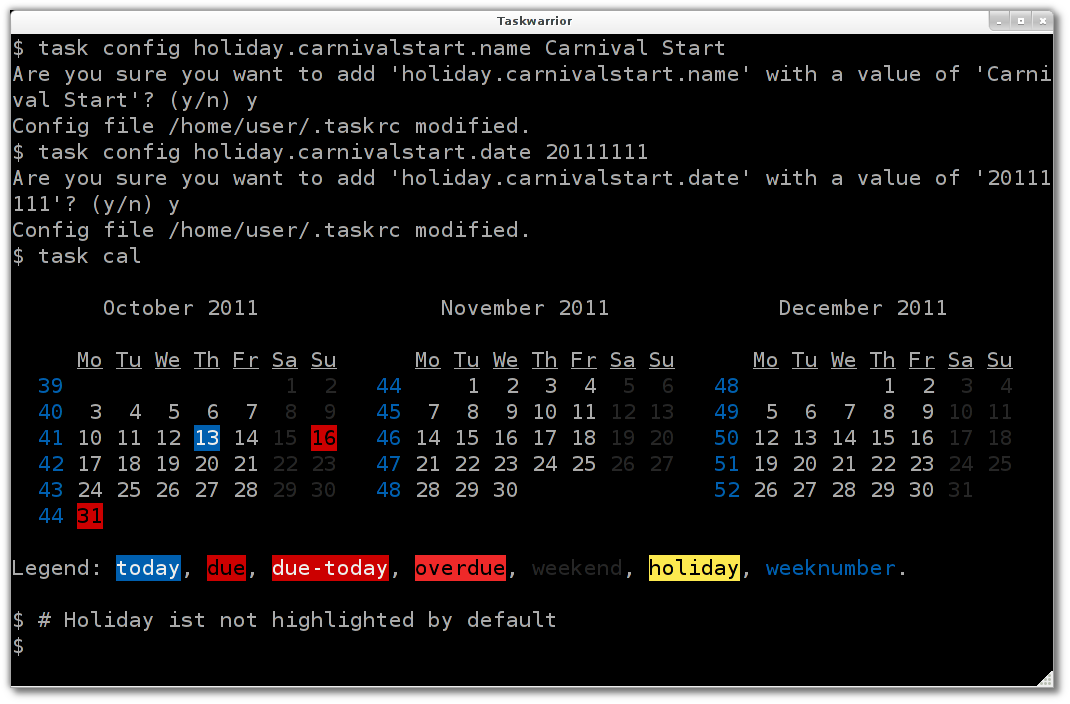
\includegraphics[width=10cm,height=7.5cm]{holiday_add.png}
\end{center}
\end{frame}

\begin{frame}
\frametitle{Calendar config with holiday}
\begin{center}
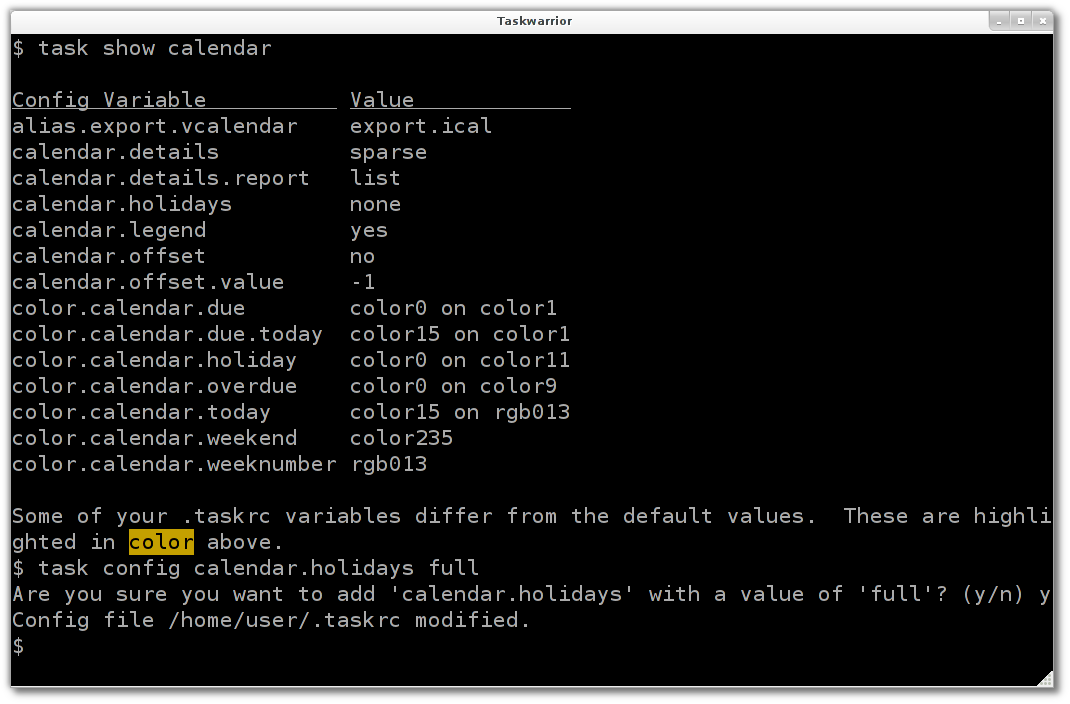
\includegraphics[width=10cm,height=7.5cm]{calendar_config_with_holiday_name.png}
\end{center}
\end{frame}

\begin{frame}
\frametitle{Calendar with holiday}
\begin{center}
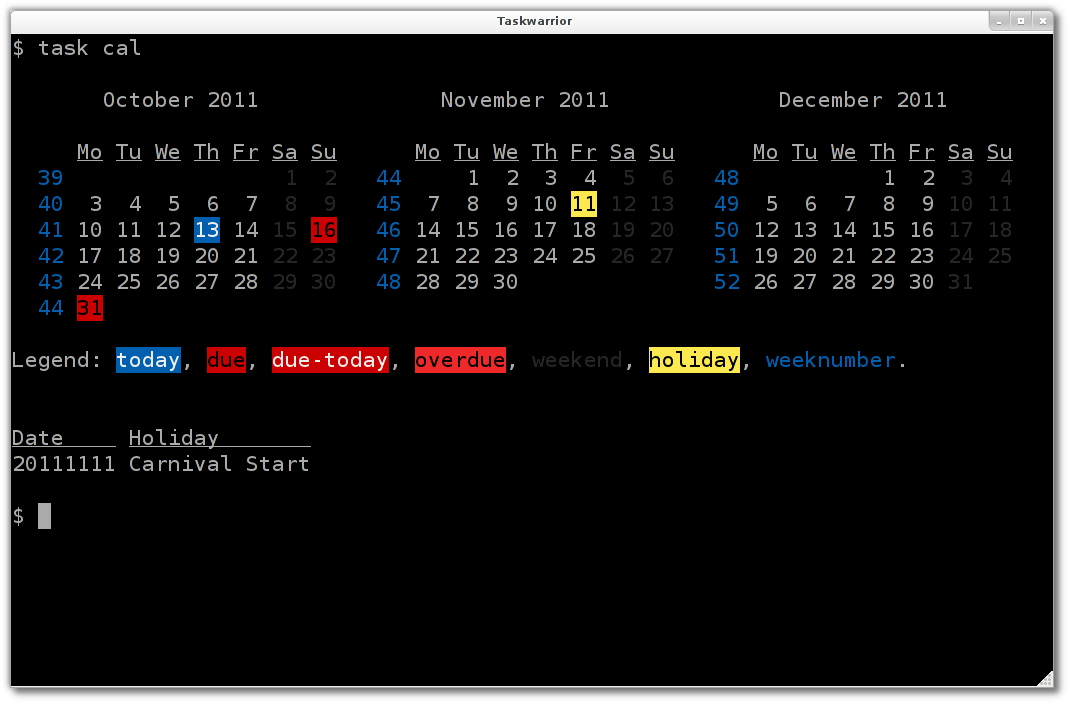
\includegraphics[width=10cm,height=7.5cm]{calendar_with_holiday_name.png}
\end{center}
\end{frame}

\begin{frame}
\frametitle{Calendar with due tasks}
\begin{center}
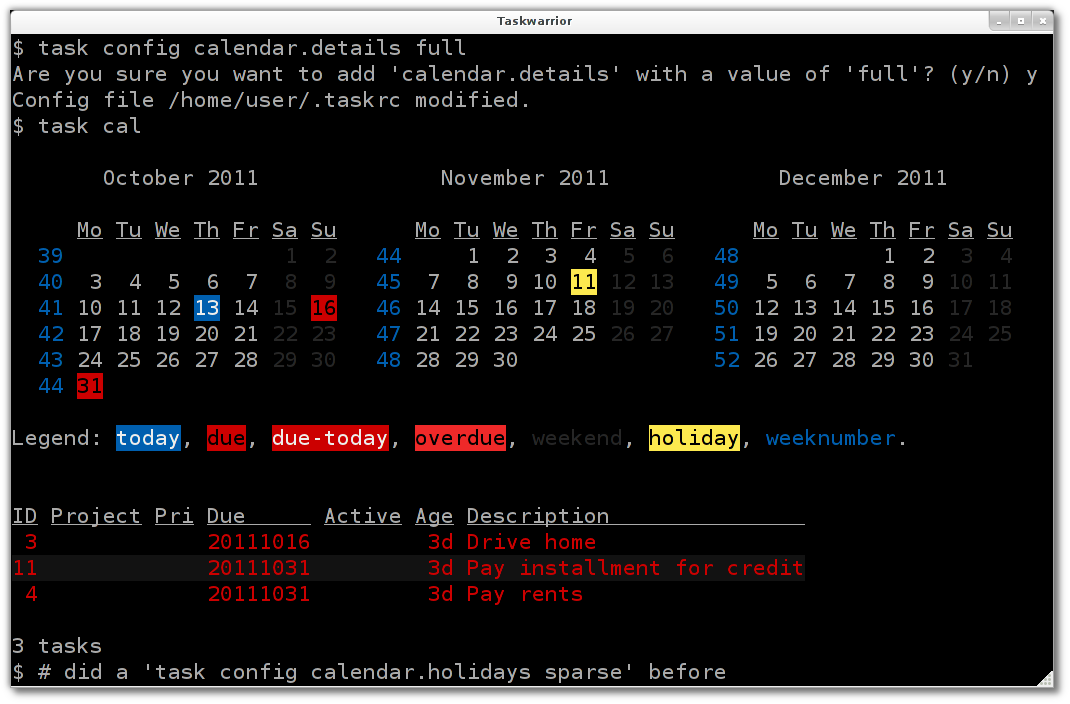
\includegraphics[width=10cm,height=7.5cm]{calendar_with_due_tasks.png}
\end{center}
\end{frame}

\begin{frame}
\frametitle{Timesheet}
\begin{center}
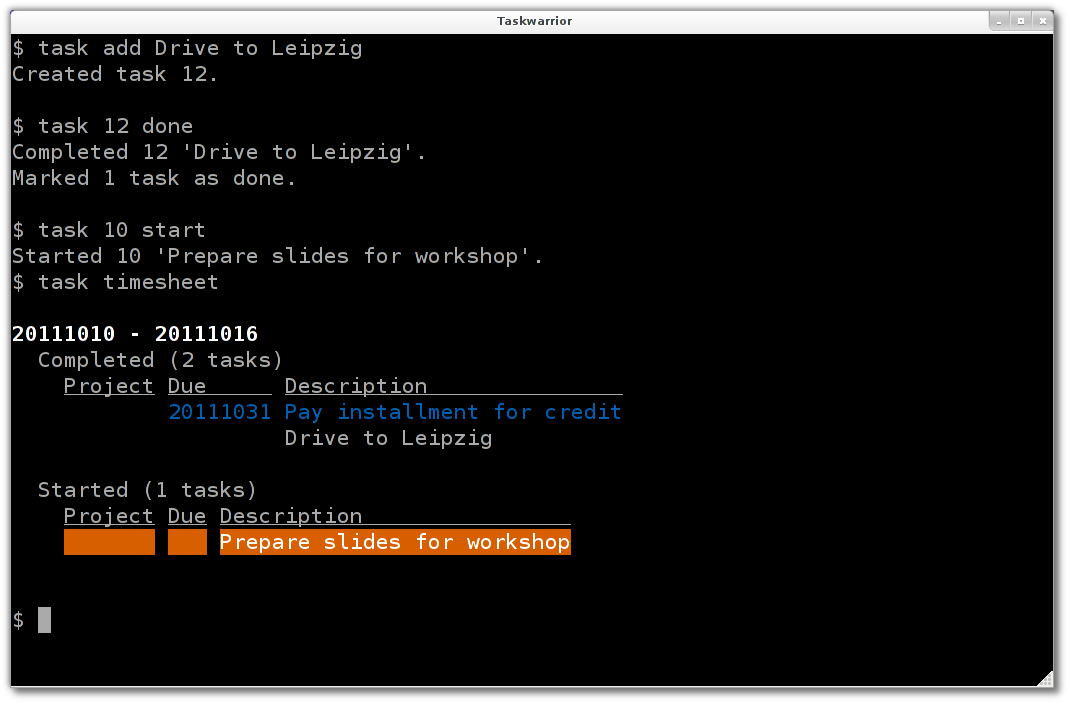
\includegraphics[width=10cm,height=7.5cm]{timesheet.png}
\end{center}
\end{frame}

\section{Getting sorted}

\begin{frame}
\frametitle{Project and subproject}
\begin{center}
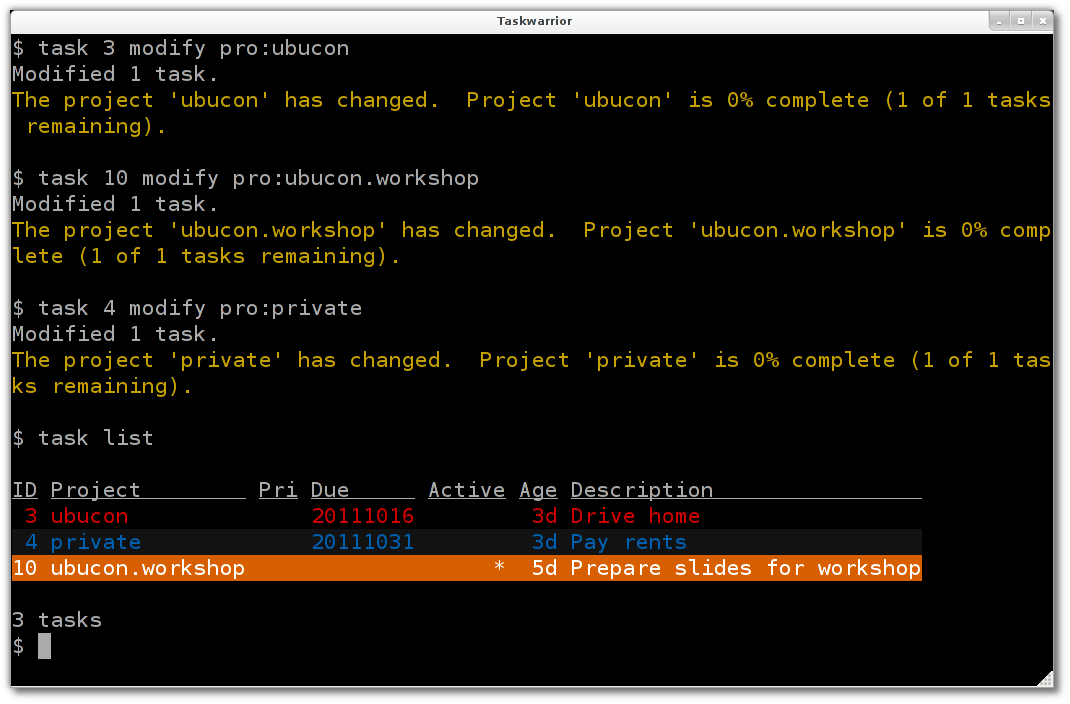
\includegraphics[width=10cm,height=7.5cm]{project_and_subproject.png}
\end{center}
\end{frame}

\begin{frame}
\frametitle{Projects}
\begin{center}
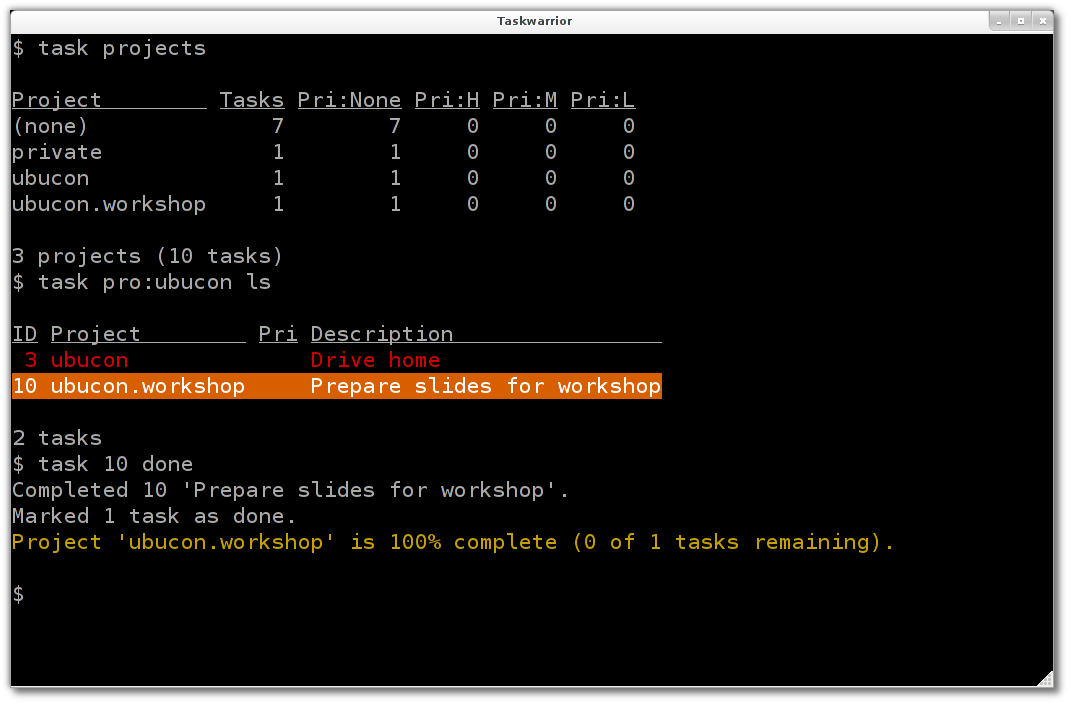
\includegraphics[width=10cm,height=7.5cm]{projects.png}
\end{center}
\end{frame}

\begin{frame}
\frametitle{Tags}
\begin{center}
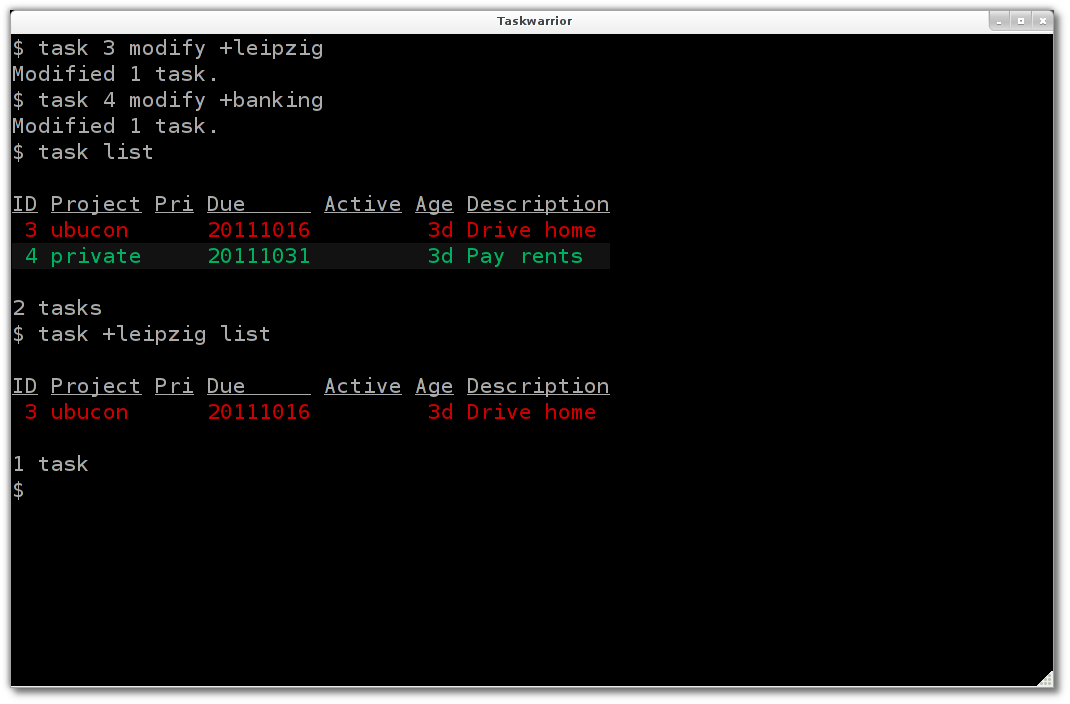
\includegraphics[width=10cm,height=7.5cm]{tags.png}
\end{center}
\end{frame}

\begin{frame}
\frametitle{Annotations}
\begin{center}
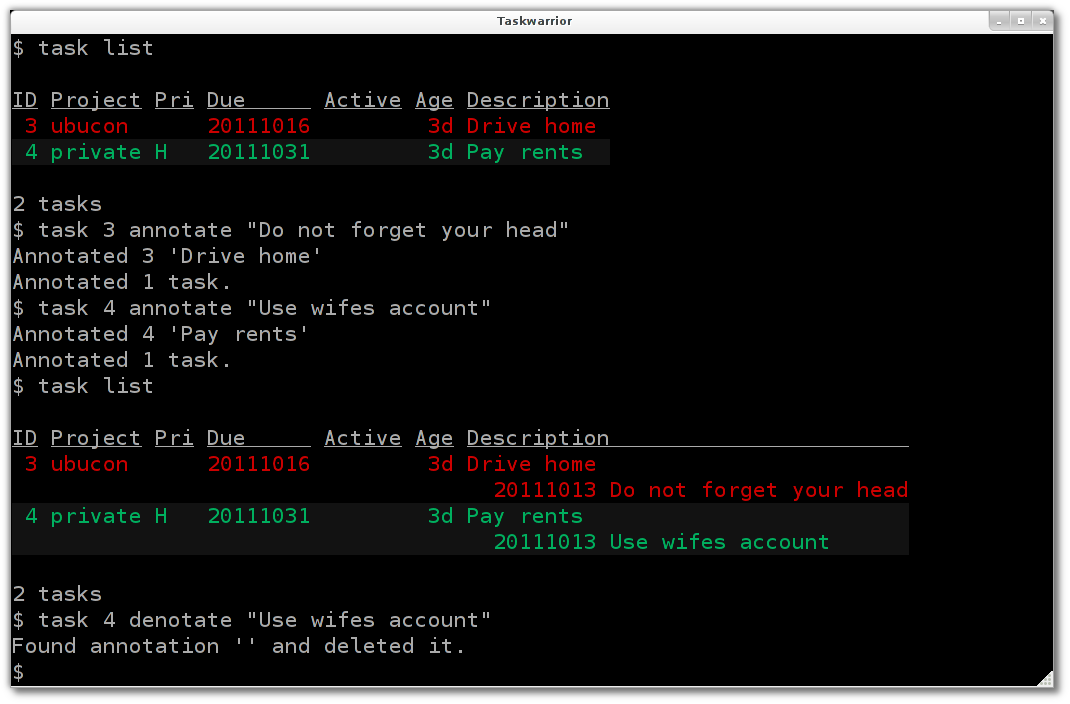
\includegraphics[width=10cm,height=7.5cm]{annotations.png}
\end{center}
\end{frame}

\section{Dependencies}

\begin{frame}
\frametitle{Dependency, part 1}
\begin{center}
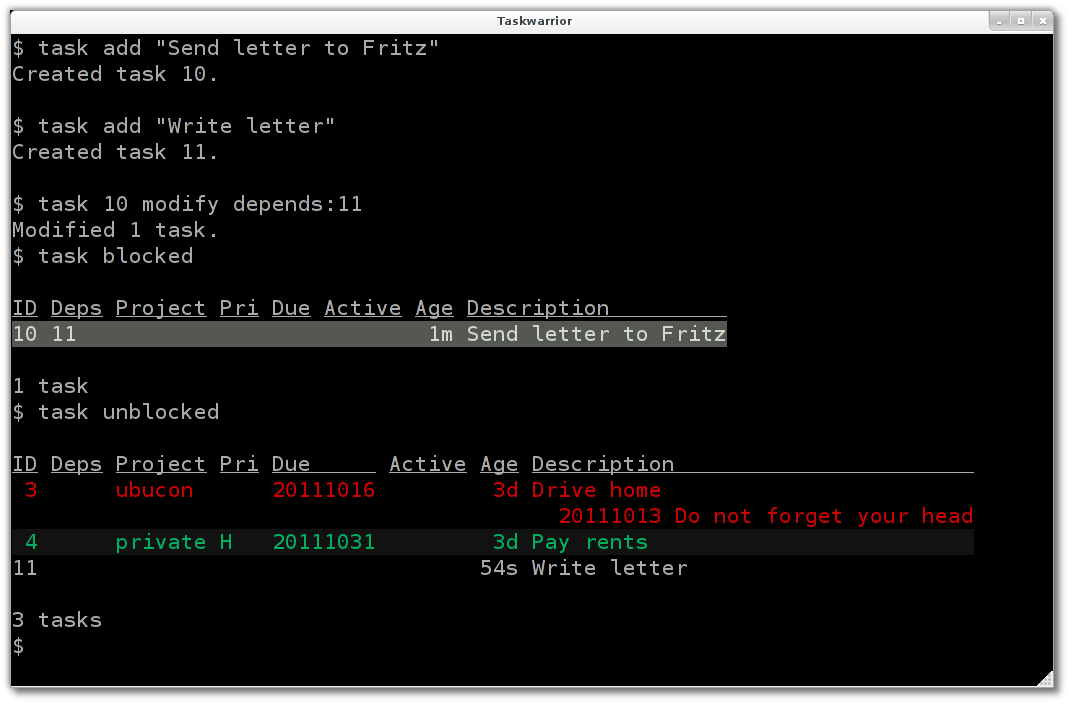
\includegraphics[width=10cm,height=7.5cm]{dependency01.png}
\end{center}
\end{frame}

\begin{frame}
\frametitle{Dependency, part 2}
\begin{center}
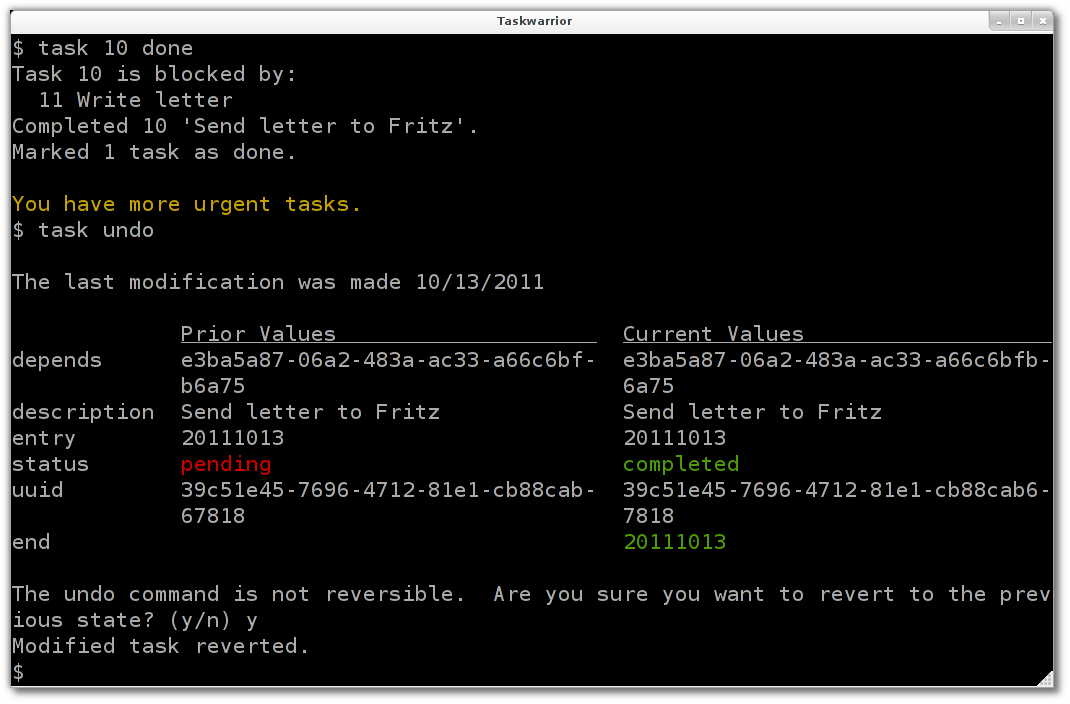
\includegraphics[width=10cm,height=7.5cm]{dependency02.png}
\end{center}
\end{frame}

\begin{frame}
\frametitle{Dependency, part 3}
\begin{center}
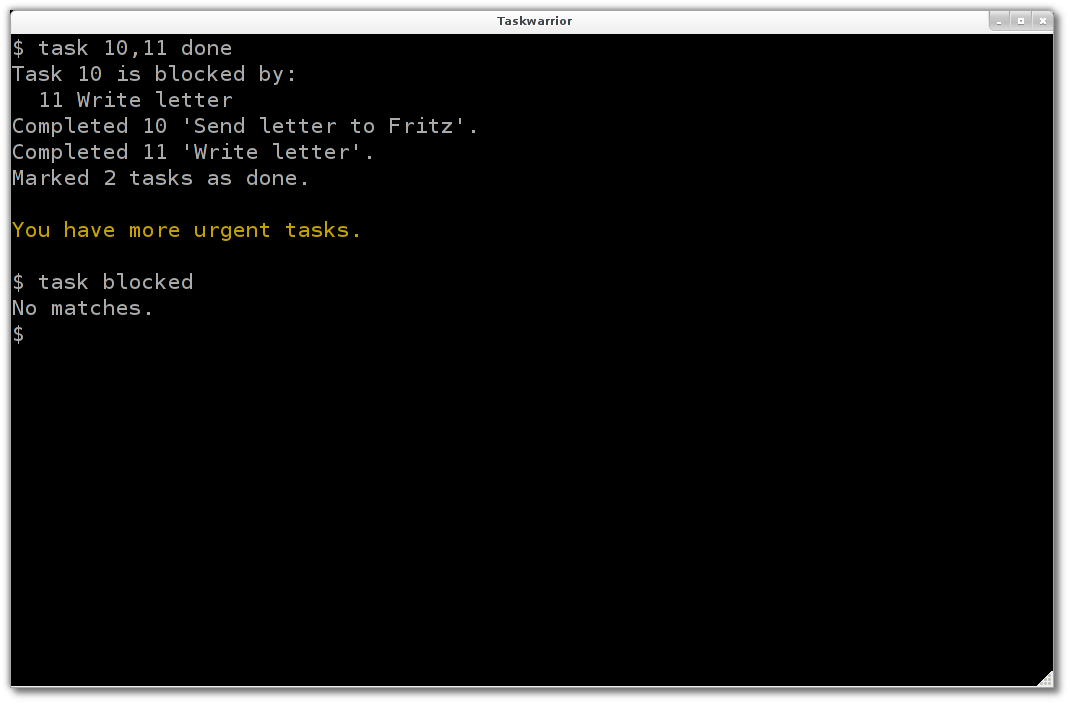
\includegraphics[width=10cm,height=7.5cm]{dependency03.png}
\end{center}
\end{frame}

\section{Reports}

\begin{frame}
\frametitle{Predefined reports (from task reports), part 2}

These reports were already used.

\begin{itemize}
\item \textbf{blocked}          Lists all blocked tasks matching the specified criteria
\item \textbf{list}             Lists all tasks matching the specified criteria
\item \textbf{long}             Lists all task, all data, matching the specified criteria
\item \textbf{projects}         Shows a list of all project names used, and how many tasks are in each
\item \textbf{recurring}        Lists recurring tasks matching the specified criteria
\item \textbf{unblocked}        Lists all unblocked tasks matching the specified criteria
\item \textbf{waiting}          Lists all waiting tasks matching the specified criteria
\end{itemize}
\end{frame}

\begin{frame}
\frametitle{Predefined reports (from task reports), part 2}

New ones:

\begin{itemize}
\item \textbf{active}           Lists active tasks matching the specified criteria
\item \textbf{all}              Lists all tasks matching the specified criteria, including parents of recurring tasks
\item \textbf{burndown.daily}   Shows a graphical burndown chart, by day
\item \textbf{burndown.monthly} Shows a graphical burndown chart, by month
\item \textbf{burndown.weekly}  Shows a graphical burndown chart, by week
\item \textbf{completed}        Lists completed tasks matching the specified criteria
\item \textbf{ghistory.annual}  Shows a graphical report of task history, by year
\item \textbf{ghistory.monthly} Shows a graphical report of task history, by month
\item \textbf{history.annual}   Shows a report of task history, by year
\item \textbf{history.monthly}  Shows a report of task history, by month
\item \textbf{information}      Shows all data and metadata for specified tasks
\item \textbf{ls}               Minimal listing of all tasks matching the specified criteria
\item \textbf{minimal}          A really minimal listing
\end{itemize}
\end{frame}

\begin{frame}
\frametitle{Predefined reports (from task reports), part 3}

And more:

\begin{itemize}
\item \textbf{newest}           Shows the newest tasks
\item \textbf{next}             Lists the most urgent tasks
\item \textbf{oldest}           Shows the oldest tasks
\item \textbf{overdue}          Lists overdue tasks matching the specified criteria
\item \textbf{summary}          Shows a report of task status by project
\item \textbf{tags}             Shows a list of all tags used
\end{itemize}

26 reports in total
\end{frame}

\begin{frame}
\frametitle{burndown.daily}
\begin{center}
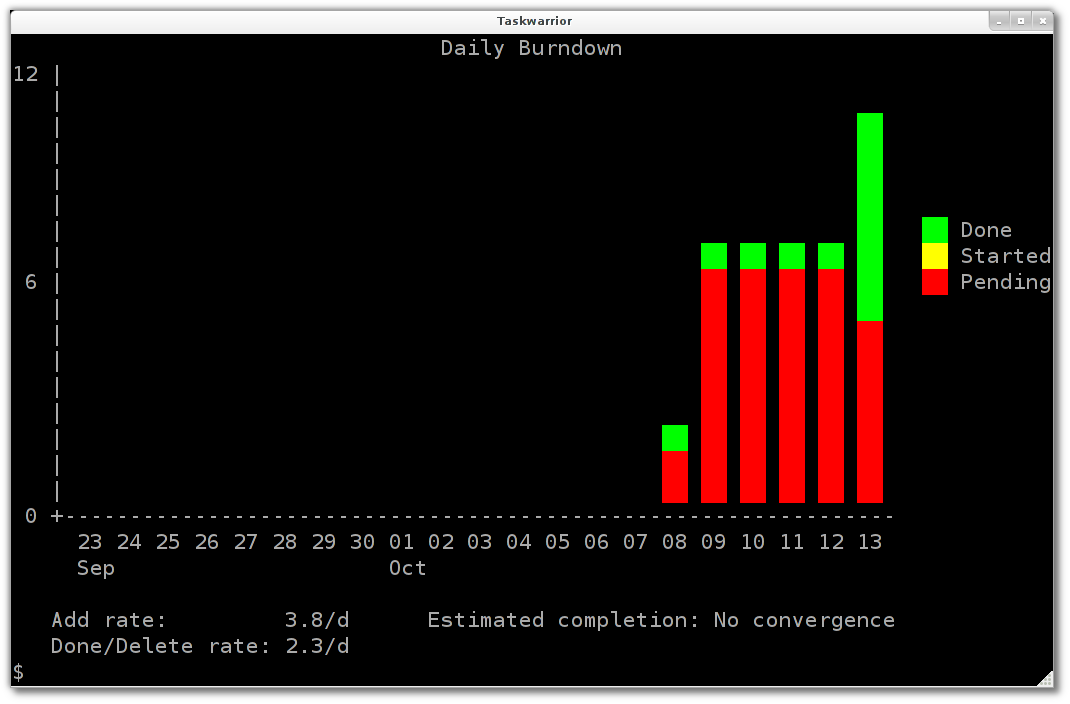
\includegraphics[width=10cm,height=7.5cm]{reports01.png}
\end{center}
\end{frame}

\begin{frame}
\frametitle{ghistory, history}
\begin{center}
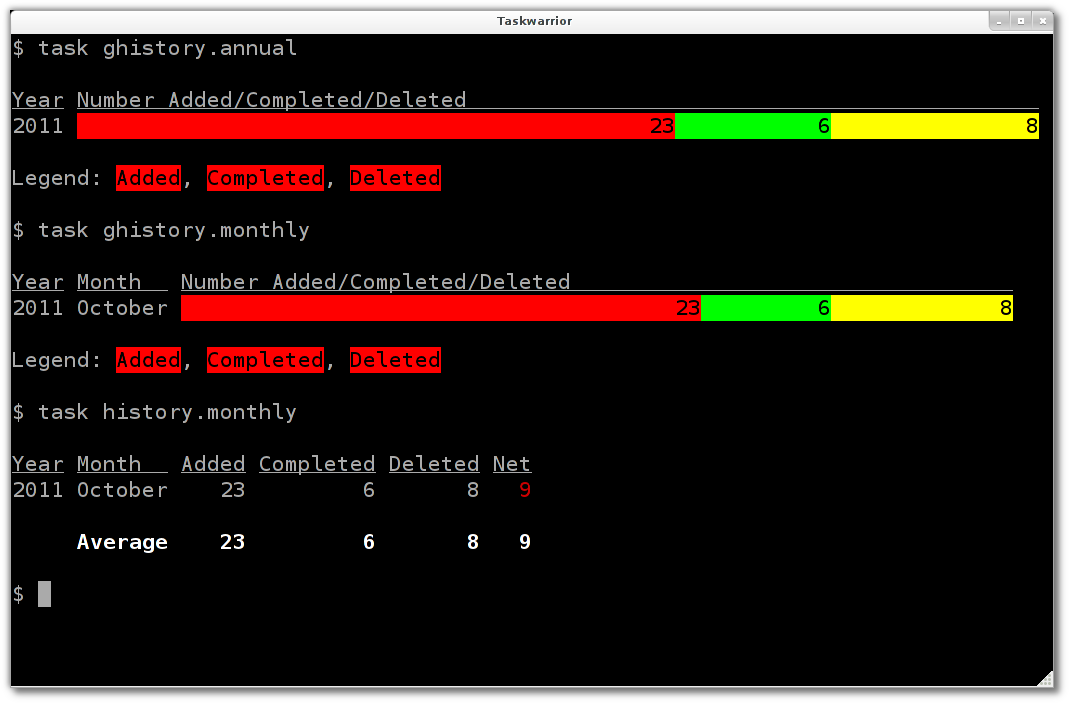
\includegraphics[width=10cm,height=7.5cm]{reports02.png}
\end{center}
\end{frame}

\begin{frame}
\frametitle{ls, minimal, summary}
\begin{center}
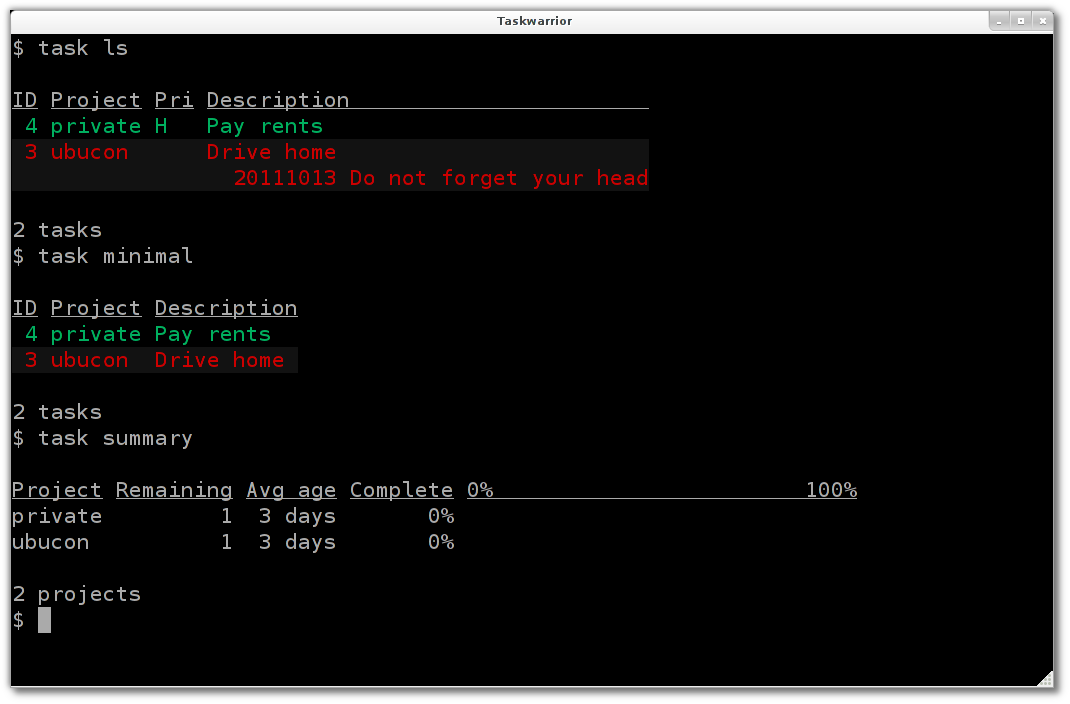
\includegraphics[width=10cm,height=7.5cm]{reports03.png}
\end{center}
\end{frame}

\begin{frame}
\frametitle{Report definitions}
\begin{center}
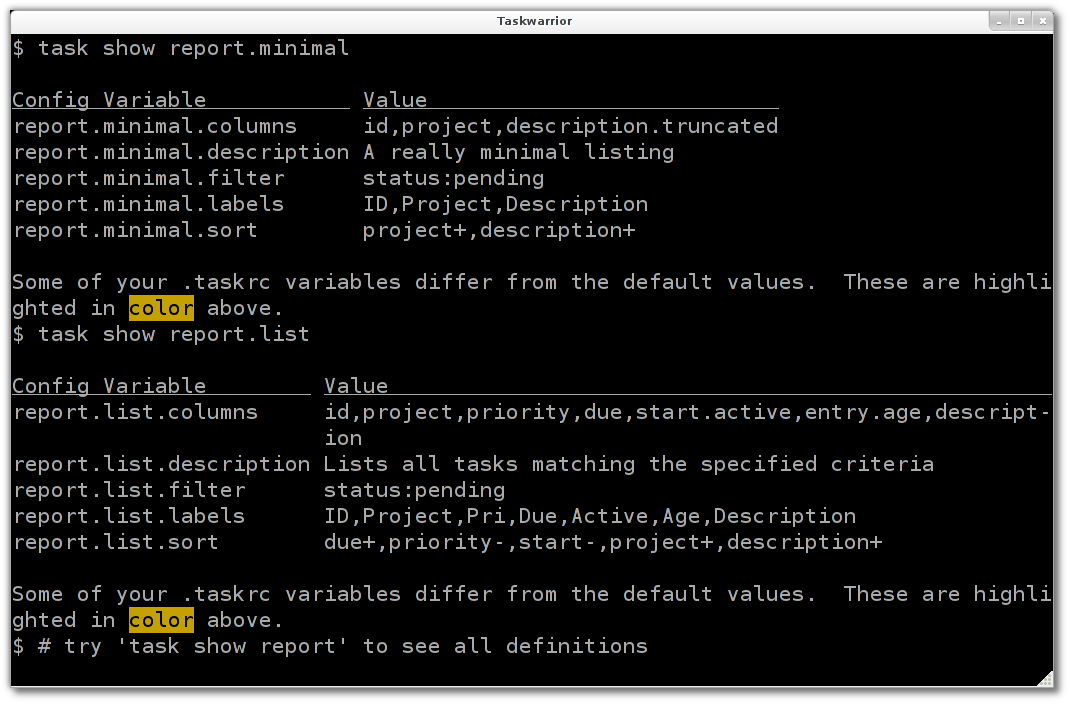
\includegraphics[width=10cm,height=7.5cm]{report_definitions.png}
\end{center}
\end{frame}

\begin{frame}
\frametitle{Dirks task list}
\begin{center}
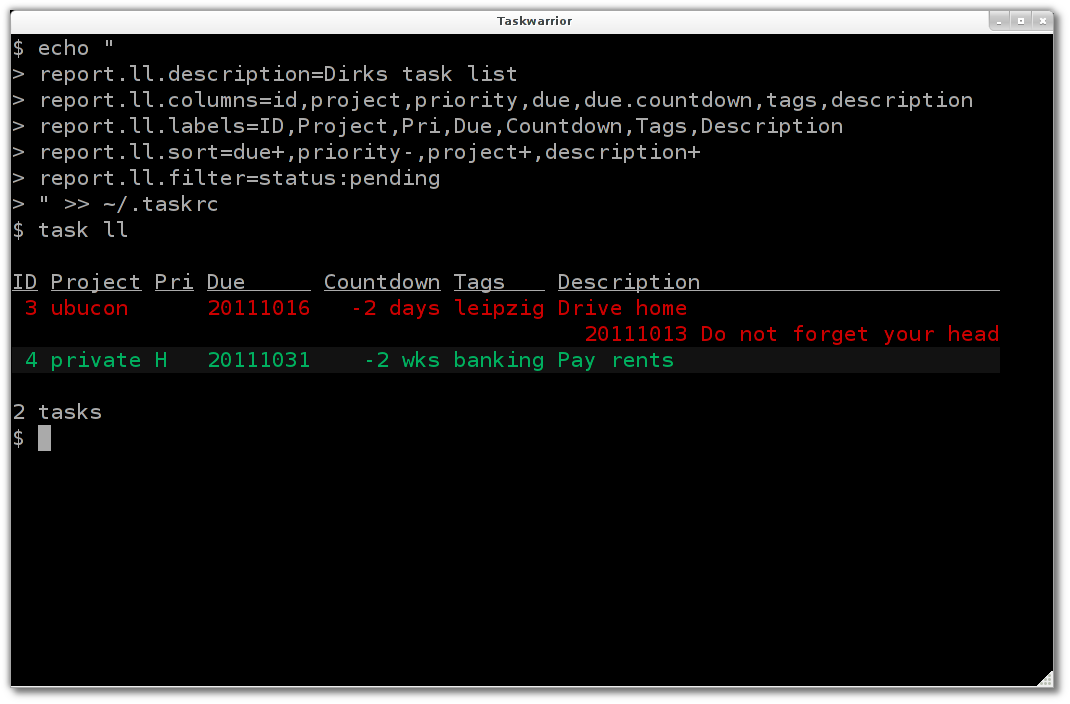
\includegraphics[width=10cm,height=7.5cm]{report_dirks_list.png}
\end{center}
\end{frame}

\begin{frame}
\frametitle{Set default command}
\begin{center}
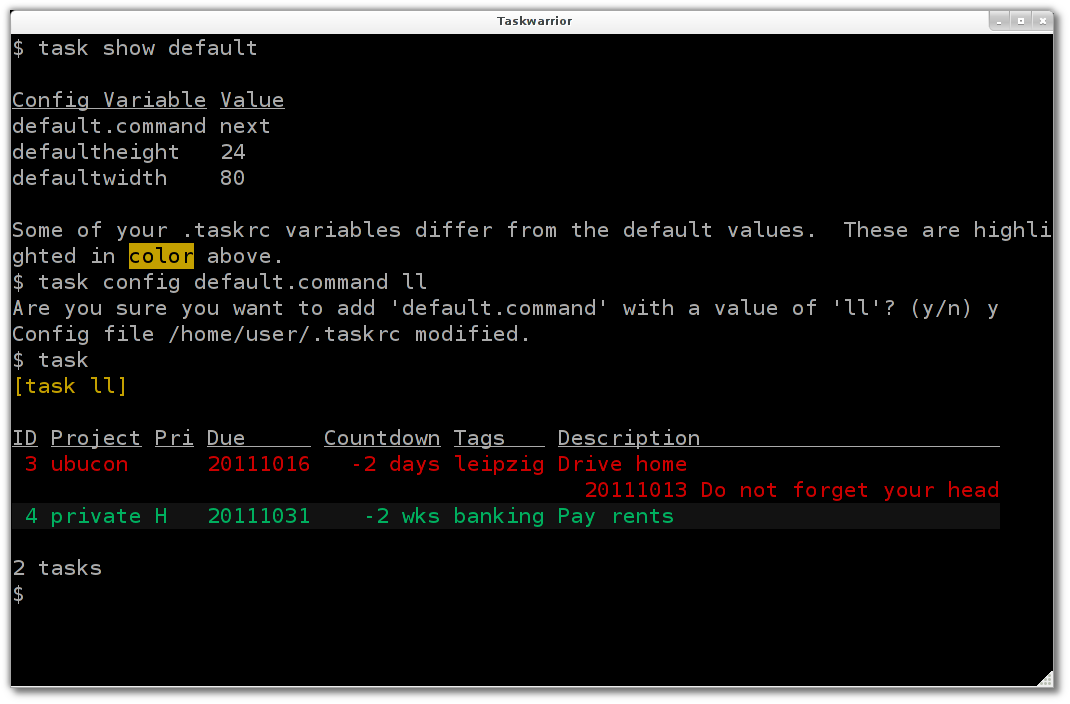
\includegraphics[width=10cm,height=7.5cm]{set_default_command.png}
\end{center}
\end{frame}

\section{Filtering}

\begin{frame}
\frametitle{Filtering in general}

You can filter for any modifier. If you don't use a modifier description is searched for the term, which may be a regular expression, on the command line. Filters may be combined.

The following attribute modifiers maybe applied as well. Names in brackets can be used alternatively.

So a filter can look like "'attribute.modifier:value"'.

\begin{itemize}
\item before, after
\item none, any
\item is (equals), isnt (not)
\item has (contains), hasnt
\item startswith (left), endswith (right)
\item word, noword
\end{itemize}
\end{frame}

\begin{frame}
\frametitle{Searches}
\begin{center}
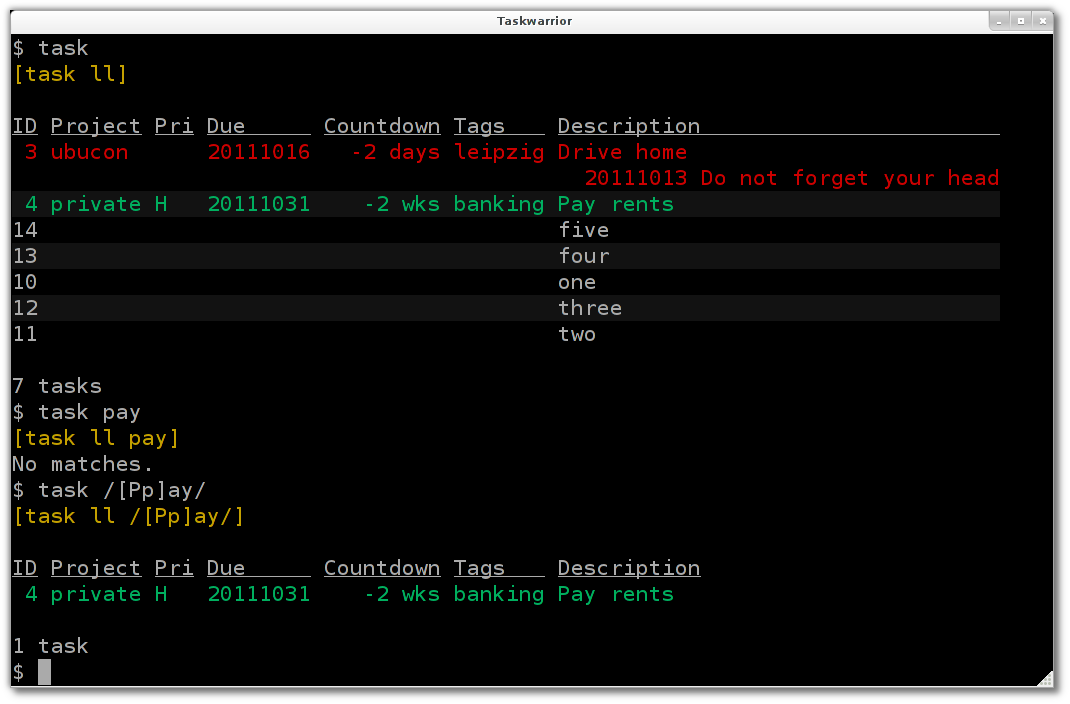
\includegraphics[width=10cm,height=7.5cm]{filter_searches.png}
\end{center}
\end{frame}

\begin{frame}
\frametitle{Attribute modifiers}
\begin{center}
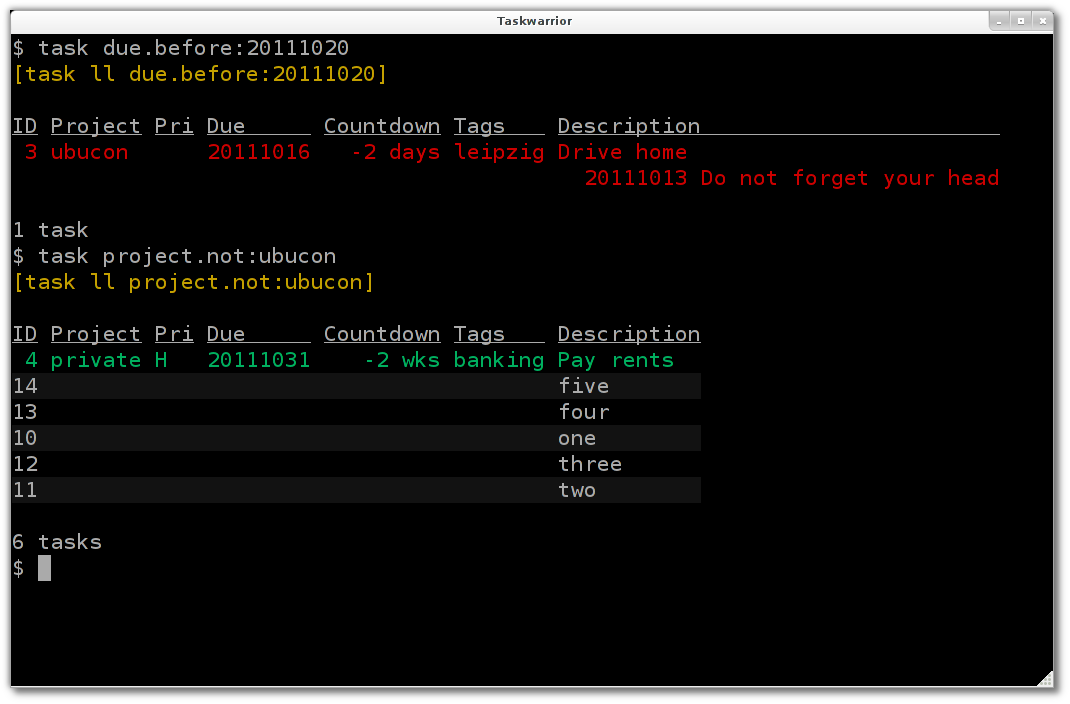
\includegraphics[width=10cm,height=7.5cm]{filter_attribute_modifiers.png}
\end{center}
\end{frame}

\begin{frame}
\frametitle{Combining}
\begin{center}
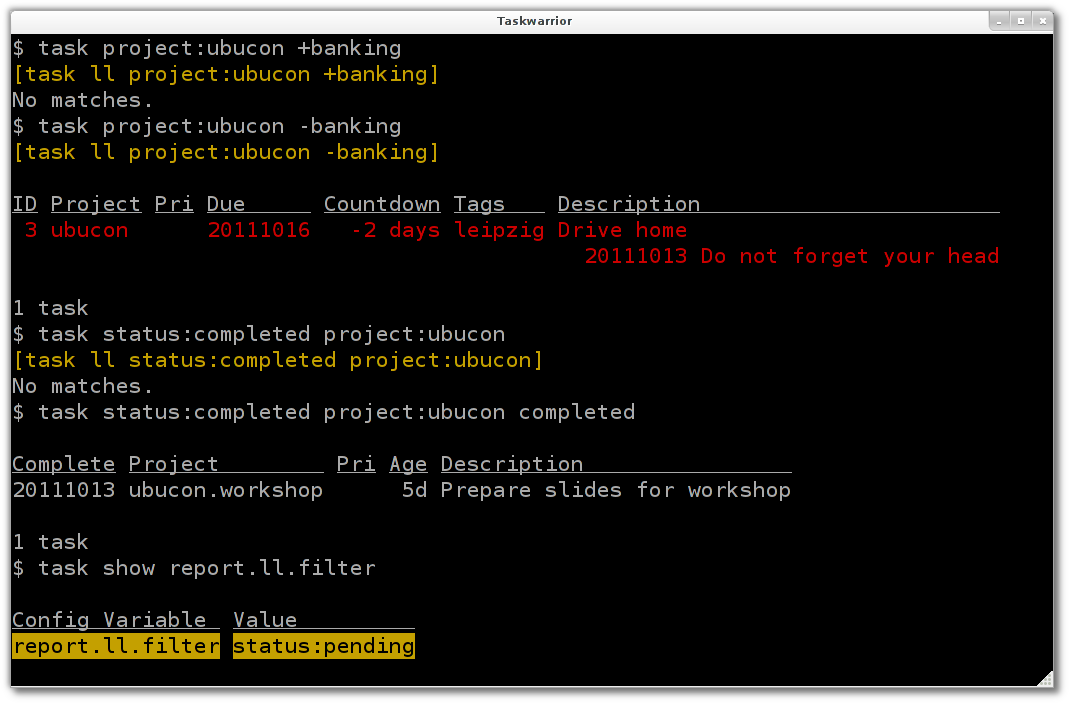
\includegraphics[width=10cm,height=7.5cm]{filter_combining.png}
\end{center}
\end{frame}

\begin{frame}
\frametitle{Or ...}
\begin{center}
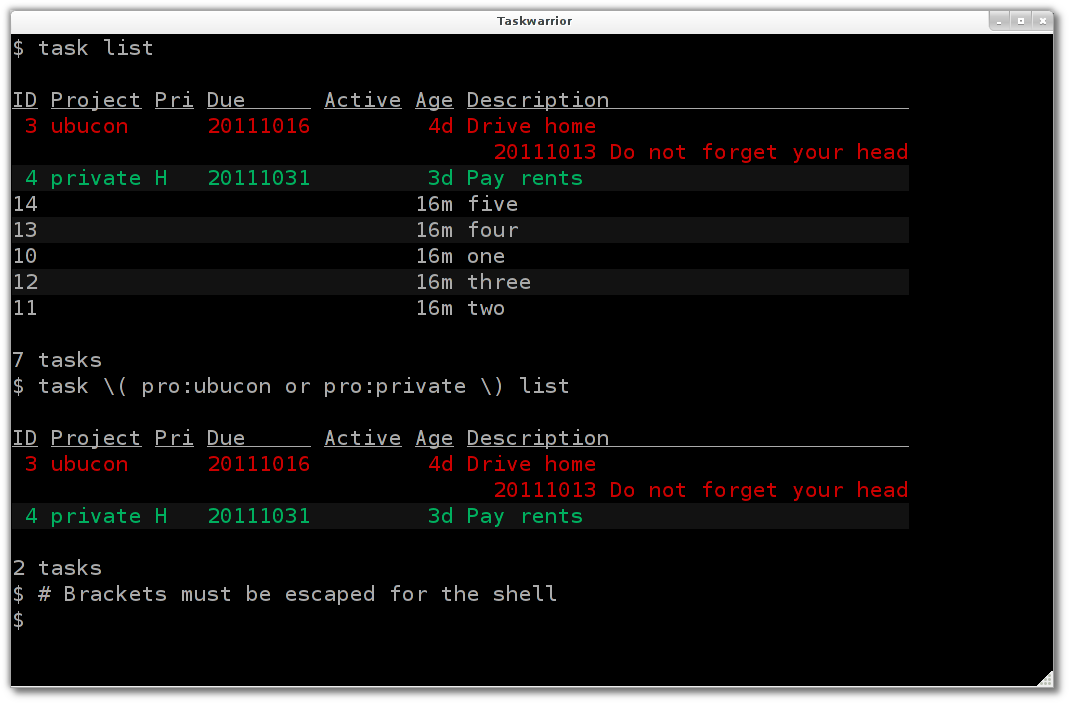
\includegraphics[width=10cm,height=7.5cm]{filter_or.png}
\end{center}
\end{frame}

\begin{frame}
\frametitle{Search configuration}
\begin{center}
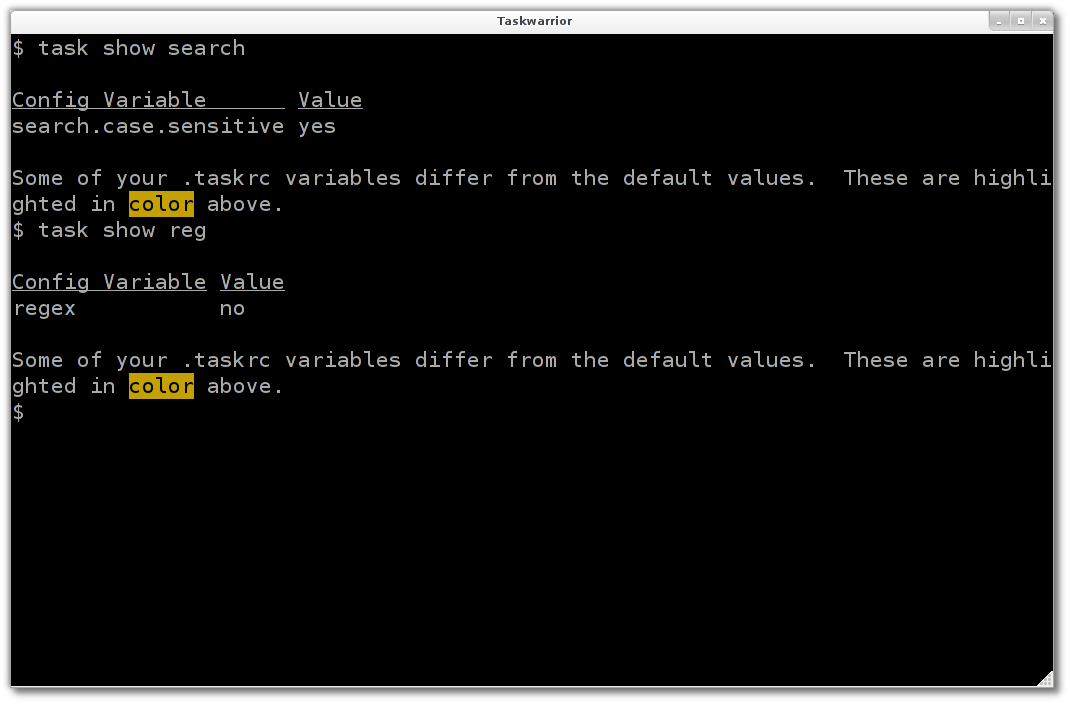
\includegraphics[width=10cm,height=7.5cm]{filter_config.png}
\end{center}
\end{frame}

\begin{frame}
\frametitle{Filter in reports}
\begin{center}
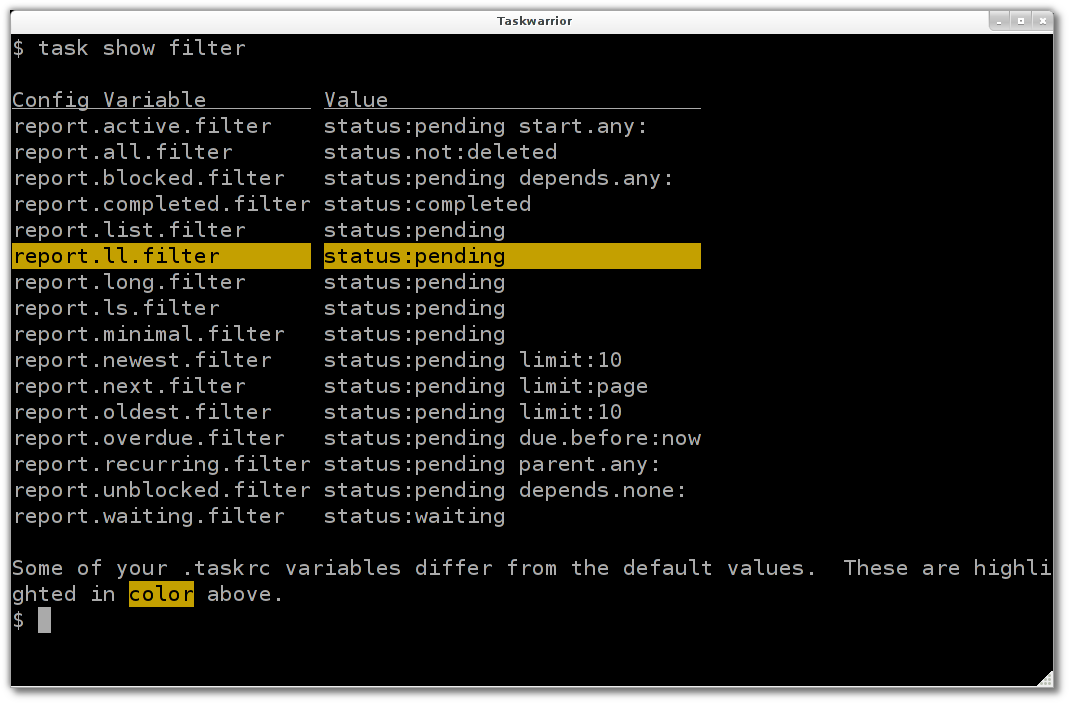
\includegraphics[width=10cm,height=7.5cm]{filter_reports.png}
\end{center}
\end{frame}

\section{Miscellanous}

\begin{frame}
\frametitle{This is by far not all}
\begin{itemize}
\item \textbf{task log}  \\
for logging a task after it is already done.
\item \textbf{task diag} \\
to help support for diagnostic purpose.
\item \textbf{task shell} \\
a simple shell to get rid of the necessity to type "'task"' all the time.
\item ... and many more!
\end{itemize}
\end{frame}

\section{That's all}

\begin{frame}
\frametitle{Questions?}
\begin{center}

\includegraphics[width=6.4cm,height=7.5cm]{task_logo.png}
\end{center}
\end{frame}

\begin{frame}
\frametitle{Support}
\begin{center}
\href{http://taskwarrior.org/}{taskwarrior.org \\ 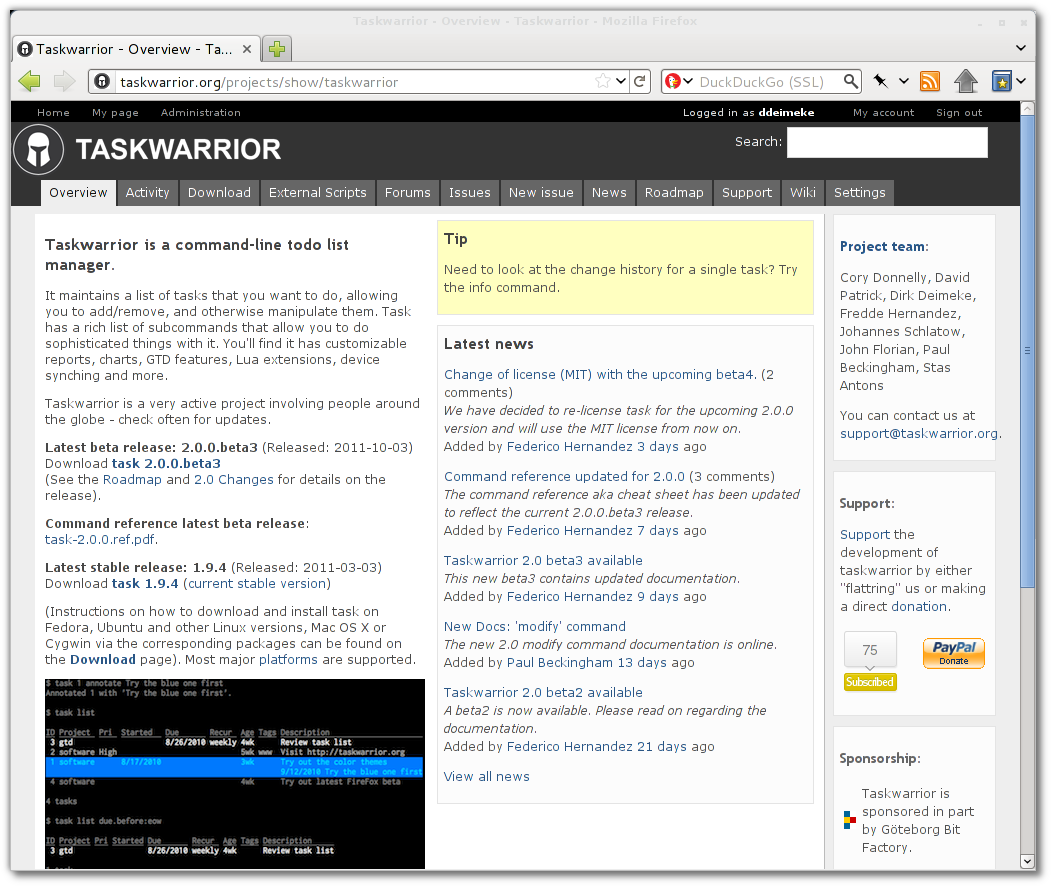
\includegraphics[width=8cm,height=6cm]{website.png}} \\
\href{mailto:support@taskwarrior.org}{support@taskwarrior.org} \\
\#taskwarrior on freenode.net -- @taskwarrior on Twitter or identi.ca
\end{center}
\end{frame}

\begin{frame}
\frametitle{Thanks for your patience!}
\begin{center}
Dirk Deimeke, Taskwarrior-Team, 2011, \href{https://creativecommons.org/licenses/by/3.0/}{CC-BY}

\href{mailto:dirk@deimeke.net}{dirk@deimeke.net}

\href{http://d5e.org/}{d5e.org} -- \href{http://dirk.deimeke.net/}{dirk.deimeke.net}
\end{center}
\end{frame}

\end{document}

%\begin{frame}[fragile]
%\frametitle{Title}
%\begin{lstlisting}
%\end{lstlisting}
%\end{frame}

%\begin{frame}
%\frametitle{title}
%\begin{center}
%\includegraphics[width=10cm,height=7.5cm]{name.png}
%\end{center}
%\end{frame}

%\begin{frame}
%\frametitle{title}
%\begin{itemize}
%\item \textbf{task {\tt<}filter{\tt>} modify}
%\end{itemize}
%\end{frame}

